%Einfache Vorlage für eine mit Latex realisierte Hausarbeit von http://www.studieren-info.de
%Du kannst diese Vorlage für deine Hausarbeit beliebig anpassen%


%-------------------
%Beginn des Kopfbereiches
%-------------------

%Wir verwenden eine DIN-A4-Seite und die Schriftgröße 12.
\documentclass [11pt,a4paper,bibliography=totoc]{scrreprt}%Einfaches Dokument{article, scrartcl} komplexere Dokumente/Studienarbeiten {report, scrreprt} Bücher {book, scrbook} Präsentationen {beamer, seminar, texpower} Briefe {g-brief, scrlttr2}

%Diese drei Pakete benötigen wir für die Umlaute, Deutsche Silbentrennung etc.
%Apple-Nutzer sollten anstelle von \usepackage[latin1]{inputenc} das Paket \usepackage[applemac]{inputenc} verwenden
\usepackage[utf8]{inputenc}%[utf8] Umlaute direkt eingabe [latin1] für unixoide und windows
\usepackage[ngerman]{babel}
\usepackage[T1]{fontenc}
\usepackage{tikz}
\usetikzlibrary{shapes,arrows}
%\usepackage{scrhack}
\usepackage[margin=9pt,font=small,labelfont=bf,textfont=it,belowskip=.3cm]{caption}
%Verwendung von vielen Farben
%\usepackage[usenames,dvipsnames]{color}
\usepackage{color}
% deutsches Literaturverzeichnis
\usepackage{bibgerm}
\usepackage{listings}%um Quellcode vernünftig einpflegen zu können
\lstset{language=C} 
\definecolor{codegreen}{rgb}{0,0.6,0}
\definecolor{codegray}{rgb}{0.5,0.5,0.5}
\definecolor{codepurple}{rgb}{0.58,0,0.82}
\definecolor{backcolour}{rgb}{0.95,0.95,0.92}
 
\lstdefinestyle{mystyle}{
    backgroundcolor=\color{backcolour},   
    commentstyle=\color{codegreen},
    keywordstyle=\color{magenta},
    numberstyle=\tiny\color{codegray},
    stringstyle=\color{codepurple},
    basicstyle=\footnotesize,
    breakatwhitespace=false,         
    breaklines=true,                 
    captionpos=b,                    
    keepspaces=true,                 
    numbers=left,                    
    numbersep=5pt,                  
    showspaces=false,                
    showstringspaces=false,
    showtabs=false,                  
    tabsize=2
}
 
\lstset{style=mystyle}


%nutzung der verlinkten formeln
\usepackage{amsmath}
%Das Paket erzeugt ein anklickbares Verzeichnis in der PDF-Datei.
\usepackage{hyperref}
%Das Paket wird für die anderthalb-zeiligen Zeilenabstand benötigt
\usepackage{setspace}

%erweitrte mathematische Tabellenformatierung
\usepackage{array}
% Grafiken verwenden
\usepackage{graphicx}
\usepackage{float}
\usepackage{struktex}
\usepackage{eurosym}
\usepackage{tabularx}
\usepackage{textcomp}
%Funktion zum skallieren
\makeatletter
\def\ScaleIfNeeded{%
\ifdim\Gin@nat@width>\linewidth
\linewidth
\else
\Gin@nat@width
\fi
}
\makeatother

%\tiny{winzig}
%\small{klein}
%\large{groß}
%\Large{bisschen größer}
%\huge{riesig}
%\Huge{Riesig}

%\textbf{Fett}
%\textit{Kursiv}
%\emph{Kursiv}	
%\textsl{schief}
%\textsc{Kapit\"alchen}
%\textsf{Sans Serif}
%\textrm{Roman}
%\texttt{Schreibmaschine}
%\textnormal{Normale Schrift}
%\underline{unterstrichen}
%\footnote{XXX}
%\includegraphics[width=80pt]{Unterschrift.jpg}

%\textcolor{white}{bla...}
%{GreenYellow, Yellow, Goldenrod, Dandelion, Apricot, Peach, Melon, YellowOrange, Orange, BurntOrange, Bittersweet, RedOrange, Mahogany, Maroon, BrickRed, Red, OrangeRed, RubineRed, WildStrawberry, Salmon, CarnationPink, Magenta, VioletRed, Rhodamine, Mulberry, RedViolet, Fuchsia, Lavender, Thistle, Orchid, DarkOrchid, Purple, Plum, Violet, RoyalPurple, BlueViolet, Periwinkle, CadetBlue, CornflowerBlue, MidnightBlue, NavyBlue, RoyalBlue, blue, Blue, Cerulean, Cyan, ProcessBlue, SkyBlue, Turquoise, TealBlue, Aquamarine, BlueGreen, Emerald, JungleGreen, SeaGreen, Green, ForestGreen, PineGreen, LimeGreen, YellowGreen, SpringGreen, OliveGreen, RawSienna, Sepia, Brown, Tan, Gray}

%Einrückung eines neuen Absatzes
\setlength{\parindent}{0em}
%Definition der Ränder
\usepackage[paper=a4paper,left=2.5cm, right=2.0cm, top=2.5cm, bottom=2.0cm]{geometry}
%anpassung der Farben der Überschriften
\addtokomafont{disposition}{\color{black}}
%Abstand der Fußnoten
\deffootnote{1em}{1em}{\textsuperscript{\thefootnotemark\ }}

\addtolength{\footskip}{-1cm}% Fußbereich 1 cm höher setzen
%section size 
%\usepackage{titlesec}
%\titleformat{\chapter}[display]
%{\normalfont%
%    \huge% %change this size to your needs for the first line
%    \bfseries}{\chaptertitlename\ \thechapter}{15pt}{%
%    \Huge %change this size to your needs for the second line
%    }
%%\titleformat*{\chapter}{\fontsize{15}{20}\selectfont}
%\titleformat*{\section}{\fontsize{13}{20}\selectfont}
%\titleformat*{\subsection}{\fontsize{12}{17}\selectfont}

%Regeln, bis zu welcher Tiefe (section,subsection,subsubsection) überschriften angezeigt werden sollen (Anzeige der überschriften im Verzeichnis / Anzeige der Nummerierung)
\setcounter{tocdepth}{2}
\setcounter{secnumdepth}{2}

%-------------------
%Ende des Kopfbereiches
%-------------------



%-------------------
%Hier beginnt der Text deiner Hausarbeit
%-------------------
\begin{document}


%Beginn der Titelseite
\thispagestyle{empty}
\begin{center}
\begin{Huge}
\textcolor{blue}{\textbf{Entwicklung und Testen eines Ultraschall-Entfernungsmessers als Vorbereitung eines Produktentwurfes}}
\end{Huge}
\rule{\textwidth}{.4pt}
\vspace{1.5cm}
% Weiter in großer Schrift

\huge{\textbf{Projektarbeit}}\\
\begin{Large}
erstellt an der\\
Fachschule für Technik des Carl-Severing-Berufskolleg\\
für Metall- und Elektrotechnik der Stadt Bielefeld\\

\includegraphics[width=100pt]{Abbildungen/CSBlogo.png}\\

Erstellt durch:\\
\vspace{12pt}
Eduard Meiser\\Omar Hachimi \\Stephan Dannat\\FET6A\\
\vspace{12pt}
in Zusammenarbeit mit der Fa. Tinkerforge\\
betreut durch\\
Herrn Simon\\
Bielefeld, \today
\end{Large}
\end{center}

\newpage
\thispagestyle{empty}
\textbf{\Large{Persönliche Erklärung}}\vspace{10pt}

Hiermit bestätigen wir, dass die vorliegende Arbeit selbstständig verfasst und keine anderen als die angegebenen Hilfsmittel benutzt wurden. Die Stellen der Arbeit, die dem Wortlaut oder dem Sinn nach anderen Werken (dazu zählen auch Internet-quellen) entnommen sind, wurden unter Angabe der Quellen kenntlich gemacht.

\vspace{50pt}


\noindent Bielefeld,\noindent\rule{4cm}{.4pt} \hfill\rule{5cm}{.4pt}\par
\hfill Eduard Meiser 

\vspace{30pt}
%\noindent\rule{5cm}{.4pt}
\hfill\rule{5cm}{.4pt}\par
%\noindent Ort, Datum
\hfill Omar Hachimi 

\vspace{30pt}
%\noindent\rule{5cm}{.4pt}
\hfill\rule{5cm}{.4pt}\par
%\noindent Ort, Datum 
\hfill Stephan Dannat 
%				Inhaltsverzeichnis
\setcounter{page}{0}
\newpage 
\pagenumbering{roman} 
\tableofcontents 
\newpage
%				Start der eigentlichen Arbeit
\newpage
\setcounter{page}{0}
\pagenumbering{arabic}

\chapter{Einleitung}
\section{Abstract}
Das Ziel des Technikerprojekt war das Entwickeln und testen eines Ultraschall-Entfernungsmessers als Vorbereitung eines Produktentwurfs. Das Ergebnis ist ein vorläufig funktionaler Prototyp deren Software noch Optimiert werden muss.
Aus den Messungen und Tests ist klar ersichtlich, dass es mit einer Kapsel funktioniert, die sowohl ein Ultraschallsignal sendet als auch empfängt. Hierbei hat sich die Ultraschallkapsel des Herstellers EKULT als die beste Kapsel herauskistalisiert, da sie weder vertauscht noch verpolt werden kann und sich somit für das Senden und Empfangen eignet.
Die Messgenauigkeiten liegen im Bereich von 4 bis 4,5\,cm. Durch einen Korrekturwert in der Software könnte die Genauigkeit auf einen Zentimeter verbessert werden.
Die Experementierumgebungen waren unterschiedliche Entfernungsmessungen mit verschiedenen Kapseln, sowie mit variabler Amplitude. Die Resultate der Forschungsarbeit sind für Tinkerforge interessant, weil sie die Grundlage für lohnende Weiterentwicklungen darlegt.




\section{Lastenheft}
\subsection{Über Tinkerforge}
Die  Tinkerforge  GmbH  wurde  Ende  2011  mit  dem  Ziel  gegründet,  die  Handhabung eingebetteter  Systeme  zu  vereinfachen.  Das  Tinkerforge  Baukastensystem  besteht  aus aktuell fast 80 verschiedenen Modulen, die vom Anwender flexibel für die jeweilige Aufgabe  kombiniert  werden  können.  Zu  den  Modulen  zählen  diverse  Sensor-  Aktor-  und Schnittstellenmodule, die alle über Hochsprachen wie C\#, Python und Java gesteuert werden können. Tinkerforge unterstützt aktuell 17 verschiedene Programmiersprachen. Sowohl Hardware als auch die Software aller Module sind OpenSource. Die Stärke des Baukastensystems  ist  aus  Anwendersicht  die  enorme  Flexibilität,  die  Einfachheit  und
die Schnelligkeit mit der Projekte realisiert werden können. Es eignet sich daher besonders im Bereich Rapid Prototyping. Daher findet das Tinkerforge Baukastensystem Anwendung in vielen Forschungsinstituten, in diversen Entwicklungsabteilungen bekannter Automobilhersteller und Ingenieurbüros.
\subsection{Motivation}
Diese Technikerarbeit soll die Grundlage zur Entwicklung eines Entfernungssensors für das Baukastensystem bilden, der auf einer Ultraschall-Entfernungsmessung basiert. Das Baukastensystem verfügt aktuell über so einen Sensor. Bei diesem handelt es sich aber im wesentlichen um ein zugekauftes Modul, welches nicht die gewünschten Leistungen liefert. Daher soll an einem zu entwerfenden Prototypen Forschung betrieben werden, um eine eigene Lösung entwerfen zu können.
\subsection{Aufgabenbeschreibung}
Innerhalb dieser Arbeit soll der Entwurf eines Prototypen des Entfernungssensors und die damit verbundene Forschung durchgeführt werden. Dabei ist durch Recherche zu erarbeiten, welche Möglichkeiten zur Realisierung zur Verfügung stehen. Durch Messungen am Prototypen soll festgestellt werden, welche dieser Möglichkeiten funktional und finanziell realisierbar sind, um ein eigenes Produkt zu erstellen. Sollte im Anschluss noch die Möglichkeit bestehen, sind die Ergebnisse in ein serienreifes Modul umzusetzen.
\newline\newline
Diverse Teilaufgaben sind zu erledigen: \newline
\begin{itemize}
\item \textbf{Recherche}\newline
Zu  Anfang  muss  recherchiert  werden,  welche  Möglichkeiten  es  gibt  mittels  Ultraschall eine Entfernung zu ermitteln und wie diese technisch umgesetzt werden können. Zusätzlich müssen die Techniker sich mit dem Tinkerforge Baukastensystem und seiner internen Funktionsweise vertraut machen.
\item \textbf{Bauteilauswahl}\newline
Abhängig  von  der  gewählten  technischen  Umsetzung  müssen  geeignete  Komponenten ausgewählt werden. Die Auswahl sollte auch unter dem Gesichtspunkten Preis, der Bauteilverfügbarkeit und der technischen Anforderungen erfolgen.\\
\item \textbf{Schaltplanentwurf und Layouterstellung}\newline
Von  Tinkerforge  wird  das  Open  Source  CAD  Programm  KiCad  verwendet.  Mit diesem Programm ist ein Schaltplan für den Prototypen und anschließend ein Leiterplattenlayout zu erstellen.
\item \textbf{Leiterplattenbestückung}\\
Die erstellte Leiterplatte wird von Tinkerforge in Auftrag gegeben. Diese muss mit den gewählten Komponenten bestückt werden. Die Tinkerforge GmbH stellt dazu die notwendigen Werkzeuge bereit.
\item \textbf{Einrichten und Einarbeitung in die Tinkerforge Toolchain}\\
Viele  Softwarekomponenten  werden  von  der  Tinkerforge  Toolchain  automatisch generiert. Um diese Nutzen zu können muss ein Linux System %in einer virtuellen Maschine
eingerichtet werden. Anschließend muss sich mit der Funktionsweise des Generators und der Softwareversionsverwaltung"Git" vertraut gemacht werden.
\item \textbf{Testsoftware und Forschung}\\
Um Messungen an der Hardware durchführen zu können gilt es Programmblöcke zu entwerfen, mit denen die einzelnen Funktionen der Baugruppen getestet werden können. So soll ermittelt werden, wie zum einen das Ultraschallsignal effektiv ausgegeben werden kann und wie sich die Signalamplitude auf die Reichweite auswirkt. Zum anderen gilt es zu recherchieren, wie das zurückkommende Signal verarbeitet werden kann. Auch soll erarbeitet werden, wie gut das Signal unter verschiedenen Bedingungen verarbeitet werden kann und ob eine zuverlässige Verarbeitungsqualität ohne großen Aufwand realisierbar ist.
\end{itemize}
\section{Management des Projektes}

\subsection{Trello}
Zur zeitlichen Planung und Übersicht des Ablaufes wurde auf das Onlinetool Trello zurückgegriffen. Dieses ist ein kostenfreies, webbasiertes Projektmanagementtool. Es ermöglicht den Gruppenmitgliedern gleichzeitig von verschiedenen Orten auf die Oberfläche zuzugreifen und Änderungen vorzunehmen. So kann ein Teilnehmer auch neue Termine mit Kennzeichnung der Fälligkeit für andere Gruppenmitglieder einfügen, oder bereits erledigte Aufgaben für alle abhaken. Auch können hier relevante Dokumente, die alle Gruppenmitglieder lesen sollen hochgeladen, und bei Bedarf noch kommentiert werden. Für die Dokumentation lässt sich an diesem System auch einfach abgleichen, zu welchen Zeitpunkten die einzelnen Aufgaben abgeschlossen wurden.
%wunderbar/zu/stark/bewertet
\subsection{Github}
Bei Github handelt es sich um einen webbasierten Online-Dienst, der Server für Entwicklungsprojekte mit einer Versionsverwaltung bereitstellt. So können alle Daten nach einer Änderung im Programm wieder hochgeladen und mit einem Kommentar versehen werden. Sollte nach mehreren Änderungen ein Problem auftreten, kann einfach auf eine ältere Version zurück gegriffen und so der Fehler eingegrenzt werden. Auch kann ein Projekt in mehrere Abschnitte aufgeteilt werden, damit mehrere Personen unabhängig voneinander daran arbeiten können. Nach der Bearbeitung können diese wieder zusammengefügt werden. Dabei ist erkennbar, welche Änderungen von wem vorgenommen wurden. So können alle Vorgänge jederzeit verfolgt werden, um eine größtmögliche Übersicht zu gewährleisten. Durch das Kommentieren der Änderungen kann die Nachvollziehbarkeit dieser ebenfalls deutlich gesteigert werden. Des weiteren ist diese Plattform gerade für Unternehmen wie Tinkerforge, die ihren Quellcode als Open-Source anbieten besonders praktisch, da den Nutzern hier alle veröffentlichten Daten direkt zur Verfügung stehen.
\section{Richtlinien zu Erstellung von Schaltplänen und Platinenlayout anhand einem ECAD-Programmpaket}

Das Open Source CAD-Programm KiCAD ist eine Anwendung zum Erstellen von Schaltplänen und elektronischen Leiterplatten. Hier lassen sich auf einfache Weise Schaltpläne erstellen und nach einer Prüfung auf fehlerfreie Verdrahtung zur vereinfachten Platinenerstellung nutzen. 

\section{Schaltplan}
Zur Signalerzeugung wurde ein Hochsetzsteller eingesetzt, um eine höhere Spannung erzeugen zu können, als auf dem System zur Verfügung steht. So höhere Amplituden auf den Sender gegeben werden, um eine höhere Signalstärke zu erreichen. Danach wird das Signal auf eine H-Brücke geleitet, diese dient dazu aus dem Gleichsignal ein Wechselsignal mit einer Frequenz von 40kHz zu generieren. Dieses Wechselsignal wird auf den Sender gegeben um das Spannungssignal in Schallwellen umzuwandeln.\\
Wird ein zurückkommendes Signal empfangen, so wandelt der Empfänger die Schallwellen in ein Sinussignal um. Dieses Signal wird auf einen nicht invertierenden Verstärker geleitet, um die Signal-Amplitude zu verstärken und anschließend durch einen Komperator in ein Rechteckiges(digitales) Signal umgewandelt. Dieses Signal wird im Prozessor verarbeitet, um aus der Zeit zwischen senden und empfangen des Signals in die Entfernung zum betreffenden Objekt umzuwandeln.\\
Beim Schaltplanentwurf gilt es auch auf gewisse Physikalische Eigenschaften von Leitungen und Bauteilen zu achten. So sollten bei Anschluss längerer Leitungen, Condensatoren zum ausfiltern eingefangener Funksignale und anderer EMV-Belastungen, angebracht werden. Auch benötigen Bauteile wie Platinen Kondensatoren an der Spannungsversorgung, um auch kleinste Schwnakungen dieser zu vermeiden.

\section{Platinenlayout}
Bei dem Entwurf eines Platinenlayouts gibt es viele Möglichkeiten ein Ergebniss zu erzielen. So können alle Bauteile so angeordnet werden, dass alle parallelen Bauteile sauber nebeneinander aufgereiht werden, und die in Reihe dazu liegenden Bauteile auch darunter angeordnet sind. So sähe die Platine zwar ähnlich eines Kontaktplanes aus, allerdings ist diese Variante aus Sicht der EMV nicht sonderlich empfehlenswert.\\
Auch können die Bauteile wie im Schaltplan in Gruppen zusammen gelegt werden und der Schaltplan auf der Platine 1:1 nachgebildet werden. Auch bei dieser Variante ergeben sich gelegentlich Probleme, was die Führung der Leitungen, und vor allem den Verlauf der Ströme angeht.\\
So sollte ein Augenmerk auf den Stromführenden Leitungen liegen. Je höher der Strom ist, desto breiter ist die Leitung auszulegen und sie sollte auch möglichst kurz gehalten werden um weniger EMV störungen zu erzeugen. Auch sollte die Rückführung (GND) günstigerweise als eigene Leiterschicht ausgeführt werden, um einen großen Leiterquerschnitt zu gewährleisten. So kann bei der Rückführung der Ströme auch das Risiko vermieden werden, durch die Bildung von größeren Schleifen Antennen zu erzeugen. Die GND Schicht sollte so wenig wie möglich unterbrochen werden, vorallem sind Unterbrechungen quer zur Stromflussrichtung zu vermeiden. Zusätzlich ist zu beachten, dass Kondensatoren meißtens zur Verringerung von Störungen nahe digitalen Bauteilen angebracht werden sollten. Die optimale Platzierung ist direkt an den Pinns, so dass die Leiterbahn mit einem höheren Querschnitt auf den Kondensator geht, und dann mit leicht verringertem Querschnitt direkt auf die Pinne des IC-Bauteils verläuft.





\chapter{Vorbereitung}
Bevor ein erster Entwurf der Schaltpläne durchgeführt werden konnte, mussten Informationen zu den zu verwendenden Bauteilen eingeholt werden, um sicherzustellen, dass diese auch die passenden Betriebsparameter haben und untereinander kompatibel sind.
\section{Recherche der Funktionsweise}
\tikzstyle{block} = [draw, fill=blue!20, rectangle, 
    minimum height=3em, minimum width=6em]
\tikzstyle{block1} = [draw, fill=blue!20, rectangle, 
    minimum height=3em, minimum width=10em]
\tikzstyle{pinstyle} = [pin edge={to-,think,black}]
\tikzstyle{input} = [coordinate]
\tikzstyle{output} = [coordinate]
\tikzstyle{line} = [ draw, dashed, line width = 0.5pt, -latex']

\begin{minipage}{0.75\textwidth}

\begin{tikzpicture}[auto, node distance=2cm,>=latex']
\begin{picture}(250,100)
\put(-38,-95){\dashbox{2.5}(220,45)[rb] {sender}}
\node [block](controller){Controller};
\node [block, right of=controller, node distance=4.5cm] (sender)  {Sender};
\node [block, above of=sender, node distance=2cm] (hochsetzsteller) {Hochsetzsteller};
\node [block, right of=sender, node distance=4.5cm] (ultraschallkapsel)  {Ultraschallkapsel};
\node [block, below of=ultraschallkapsel, node distance=2.5cm] (filterung)  {Filterung};
\node [block, left of=filterung, node distance=4.5cm] (verstaerker)  {Verstaerker};
\node [block, left of=verstaerker, node distance=4.5cm] (komperrator)  {Komperrator};

\draw [->] (controller) -- node[name=PWM ] {$PWM$}  (sender);
\node [output, right of=sender] (output) {};
\coordinate [below of=PWM] (tmp);
\draw [->] (hochsetzsteller) -- node[name=VBB ] {$VBB$}  (sender);
\node [output, above of=sender] (output) {};
\coordinate [below of=VBB] (tmp);
\draw [->] (sender) --  (ultraschallkapsel);
\draw [->] (ultraschallkapsel) --  (filterung);
\draw [->] (filterung) --  (verstaerker);
\draw [->] (verstaerker) --  (komperrator);
\node [output, right of=sender] (output) {};
\coordinate [below of=PWM] (tmp);
\draw [->] (komperrator) --  node[name=Digital ] {$Digital$} (controller);
\node [output, above of=komperrator] (output) {};
\coordinate [below of=Digital] (tmp);
\path[line] (verstaerker)--node[name=analog] {$Analog$}  (controller);
\end{picture}
\end{tikzpicture}
\captionof{figure}{Blockschaltbild}
\label{fig:Blockschaltbild1}
\end{minipage}

Das Blockschaltbild, siehe Abbildung\ref{fig:Blockschaltbild1}, zeigt eine vereinfachte Funktionsübersicht. Der Schaltplan befindet in den Anlagen.

\subsection{Controller}
Der Controller soll eine stabile PWM ausgeben können sowie die Berechnung; Analaog und Digital, der Entfernungsmessung beherrschen. Die Ausgabe der Entfernung erfolgt an einer Universellen-Schnittstelle. 
\subsection{Hochsetzsteller}
Der Hochsetzsteller dient dazu, aus den 5V Versorgungsspannung eine (für die Versuche variable) höhere Spannung für den Sendebetrieb zu schaffen. So kann der Schalldruck der ausgegeben wird erhöht werden(größere Reichweite/größeres Rücksignal)\\
Die Funktionsweise des Hochsetzstellers (Spannungspumpe/Aufwärtswandler/Aufwärtsregler) ist relativ simpel und findet in vielen Bereichen Anwendung. Grundsätzlich wird eine Induktivität in Reihe mit einer Freilaufdiode vor einen Ladecondensator geschaltet. Dieser liegt parallel zum Ausgang. Zwischen der Spule und der Diode ist ein Schalter angeschlossen, der die Spule gegen Masse schaltet. So läd sich die Spule bei Betätigung des Schalters auf (durch den Stromfluss entsteht ein Magnetfeld) und beim Öffnen steigt die Spannung am sekundären Ende der Spule, durch das zusammenbrechende Magnetfeld, an und läd den Kondensator auf. Dieser Vorgang wird wiederholt, bis der Kondensator so weit aufgeladen ist, dass die Ausgangsspannung den gewünschten Wert hält. Dann wird die Schaltfrequenz auf das mindestmaß verringert, um den Wert zu halten. Natürlich ist die mögliche Ausgangsspannung nicht unbegrenzt über das Schaltspiel regelbar, sondern ist auch von den Baugrößen der Bauteile abhängig. Mit einer Induktivität von 10mH und einem Kapazität von 40uF lässt sich die Ausgangsspannung bei 5v Eingangsspannung zwischen 6v und 20v einstellen.
\subsection{Sender}
Der Sender soll Schallwellen im Ultraschallbereich aussenden, die einen ausreichenden Schalldruck haben, um von Hindernissen, die bis zu mehrere Meter entfernt sind ein Echo erhalten zu können.
Dafür muss die Lautsprecherkapsel mit einem Sinusähnlichen Signal angesteuert werden, dessen Amplitude angemessen hoch ist, um den gewünschten Schalldruck zu erzeugen. Mit dem Mikrocontroller kann ein Rechtecksignal erzeugt werden, bei dem die Pulsweite variierbar ist (PWM). Der Nachteil ist, dass der Mikrocontroller nur auf seine Spannungsebene von 3,3V begrenzt ist und durch höhere Spannungen zerstört würde.
Um höhere Spannungen an der Lautsprecherkapsel realisieren zu können, muss ein weiteres Bauteil dazwischen geschaltet werden. Dieses zusätzliche Bauteil dient als Trennung zwischen den 3,3V des Mikrocontrollers und der höheren Spannungsebene der Lautsprecherkapsel. Dabei wird darauf zu achten sein, dass dieser Schalter schnell genug arbeitet, um die 40kHz (Frequenz von Ultraschall) auch sauber schalten zu können.
\subsection{Empfänger}
Im Empfangsbetrieb werden die zurückkommenden Schallsignale, die auf die Lautsprecherkapsel treffen in Sinusförmige Spannungssignale umgewandelt. Die Amplitude dieser Signale hängt von dem Schalldruck der empfangenen Signale ab und ist deutlich nieriger als die Amplitude der gesendeten Signale. Diese Signale müssen anschließend verstärkt werden, um sie mit dem Mikrocontroller auswerten zu können. Zur Vereinfachung der Auswertung macht es auch Sinn, das eingehende analoge Signal in ein Digitales Signal umzuwandeln, dies kann einiges an Verarbeitungsaufwand einsparen. Um die qualität der gemessenen Entfernung besser zu beurteilen sollte auch das Analogesignal ausgewertet und verglichen werden mit dem umgewandelten Digitalen Signal. Es dient unteranderem nämlich dazu wie die spätere Software auszusehen hat, denn die Auswertung eines Analogensignals erfordert mehr Programmieraufwand als die Auswertung eines Digitalensignals. Um ein Digitales Signal auszuwerten reicht es im Grunde genommen auf den ersten Impuls zu warten, die Wartezeit wird in die entfernungsmessung mit einbezogen und somit ergibt sich die Entfernung. Bei der Analogen Auswertung muss mit dem gesendet mit dem empfangenen Signal verglichen und überprüft ob es sich um die 40kHz handelt oder nur eine Störung ist.
Mit der Zeit, die zwischen dem gesendeten Signal und dem empfangenen Signal vergeht, muss letztendlich der Abstand zwischen dem Sensor und dem Hinderniss berechnet werden.
\subsection{Filter}
Die Fitlerschaltung soll am Eingang des Empfängers mögliche Störfrequenzen herrausfiltern um eine Verfälschung der gemessenen Strecke zu vermeiden, da die Lautsprecherkapsel nicht ausschließlich Ultraschallsignale aufnimmt.

\section{Verwendete sowie Dimensionierung der Bauteile}
Bevor ein erster Prototyp erstellt werden konnte, mussten die richtigen Bauteile ausgewählt werden. Dies Geschah unteranderem anhand der gewonnenen Informationen aus dem Kapitel 2 Vorbereitung. 

\subsection{Mikrocontroller}
Der Infineon XMC 1404\_Q048 gehört zur Familie der ARM Cortex -M0 Prozessoren und ist ein 32~Bit Industrial Mikrocontroller, wird mit 48~MHz externer Clock betrieben. Die Q048 im Namen steht für die Anzahl der Pins. Der interne Timer läuft mit 96~MHz. Die CCU4 des Prozessors bietet ein 2x4 16~Bit Timer. Zudem hat der XMC einen 12~Bit A/D Wandler, welcher für die Analogmessung eine genauere Auflösung bieten kann als ein 8~Bit A/D Wandler. Die Betriebsspannung des Prozessors beträgt 3,3~V. Die Auswahl des Mikrocontrollers wurde getroffen, weil dieser standardmäßig bei Tinkerforge eingesetzt wird und uns für den Prototypen vorgegeben wurde. 


\subsection{Sender}Um eine Trennung zwischen der Mikrocontroller, (3,3~V) und dem Hochsetzsteller (5~V-20~V)zu ermöglichen, benötigte zusätzlich ein weiteres Bauteil. Dafür wurde das IC A5950 (Voll Brücke) ausgewählt. Diese H-Brücke kann eine angeschlossene Last mit der vom Hochsetzstellers erzeugten Spannung versorgen. Deren Frequenz wird über das Signal an dem Pin \glqq Phase \grqq~von dem Prozessor vorgegeben. An den Anschlüssen Out1 und Out2 wird das Ausgangssignal abgegriffen. Für die genaue Beschaltung des ICs siehe Anhang Datenblatt  \glqq Schimatic A5950 \grqq.




\subsection{Hochsetzsteller}
Tinkerforge nutzt schon eine Variante eines Hochsetzstellers auf ihren Platinen. Der Aufbau und die Bauteilauswahl mussten nur auf die variable Ausgangspannungs erweitert werden. Die Standardschaltung, von Tinkerforge, wurde an dem Eingang der Feedbackspannung mit einem Potentiometer (RV1) ergänzt, um die gewünschte variable Spannung zu generieren.\\
Die Ausgangsspannung wird mit den externen Widerständen RV1, R13 und R2 eingestellt (siehe Grundschaltung Datenblatt vom IC LRM62014x, Seite 11). Ein Wert von ca. \(\displaystyle 13,3~k\Omega \) wurde für R2 empfohlen. Mit den Potentiometer (RV1) lässt sich die Ausgangsspannung bei 5~V Eingangsspannung bis 21,5~V einstellen. In der Formel werden die Widerstände RV1 und R13 zum Ersatzwiderstand(Re) zusammengefasst.
\onehalfspacing \\
\[\displaystyle Re=R2*\left(\frac{Vout}{1,23}-1\right) \Rightarrow Vout=\left(\frac{Re}{R2}+1\right)*1,23\] 
\singlespacing
\begin{center}
\begin{minipage}{1\textwidth}
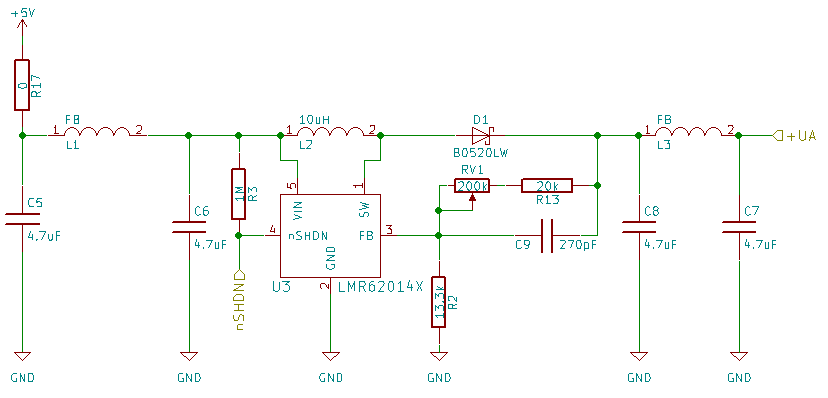
\includegraphics[width=1\textwidth%, draft
]{Abbildungen/Pumpe.png}
\captionof{figure}{Schaltplan des beschalteten Hochsetzstellers}
\label{fig:Hochsetzsteller}
\end{minipage}\\
\end{center}

\subsection{Ultraschallkapsel}%bearbeiten
Für den Prototypen wurden mehrere Kapseln diverser Hersteller bestellt. Dieses geschah um Unterschiede der verschieden preisigen Bauteile zu ermitteln und um festzustellen, welches Preissegment die nötige Qualität für die vorliegende Anwendung erfüllt.


\subsection{Filter}%bearbeiten
Um unerwünschte Signalanteile mit Frequenzen, die unter 40~kHz liegen, zu unterdrücken musste die Filterschaltung mit einem Hochpassfilter (CR Glied) bestehend aus einem Kodensator und einem Widerstand bestückt. Der Widerstand wurde nach der e24 Reihe ausgewählt.
Die Kapazität des Kondensators wurde an die Grenzfrequenz von 40~kHz und den Widerstand angepasst.
\onehalfspacing \\
\[\displaystyle C=\frac{1}{2*pi*fg*R}\Rightarrow\frac{1}{2*pi*40~kHz*100~K\Omega}\approx40~pF \]
\singlespacing
Anhand der Berechnung wurde für den Hochpassfilter ein Kondensator mit \(\displaystyle 39~pF\) genommen.

\subsection{Empfänger}
Die Abbildung \ref{fig:Empfängerschaltung} zeigt die Empfängerschaltung. Durch diese Verschaltung von Operationsverstärkern wird das ankommende sinusförmige Signal verstärkt und in ein digitales Signal umgewandelt. Für die Verstärkung der Amplitude und der Umwandlung des analogen Signals in ein Rechtecksignal mit 40~KHz wurde der das IC TLC272 ausgewählt, weil dieser günstig im Stückpreis ist und die technischen Spezifikationen ausreichend sind. Siehe Datenblatt vom IC TLC272.\\

Für die Verstärkung der Amplitude ist der Operationsverstärker TLC272 U2B als nicht invertierender Verstärker geschaltet.
Für die Umwandlung des analogen Signales in ein digitales wurde der Operationsverstärker TLC272 U2C als Komparator geschaltet. Beim Auftreten von Differenzen zwischen den Eingangssignalen, wechselt der Ausgang des Komparators zwischen Low (0~Volt) auf High (3,3~Volt).\\ Die Referenzspannung (\(\displaystyle Uref)\)  wird durch den Spannungsteiler R9 und R8 bestimmt.
\onehalfspacing \\
\[\displaystyle Uref=\frac{Uges*R9}{R8+R9}\Rightarrow\frac{3,3~V*120~K\Omega}{100~K\Omega+120~K\Omega}=1,8~V \]
\singlespacing
\begin{center}
\begin{minipage}{1\textwidth}
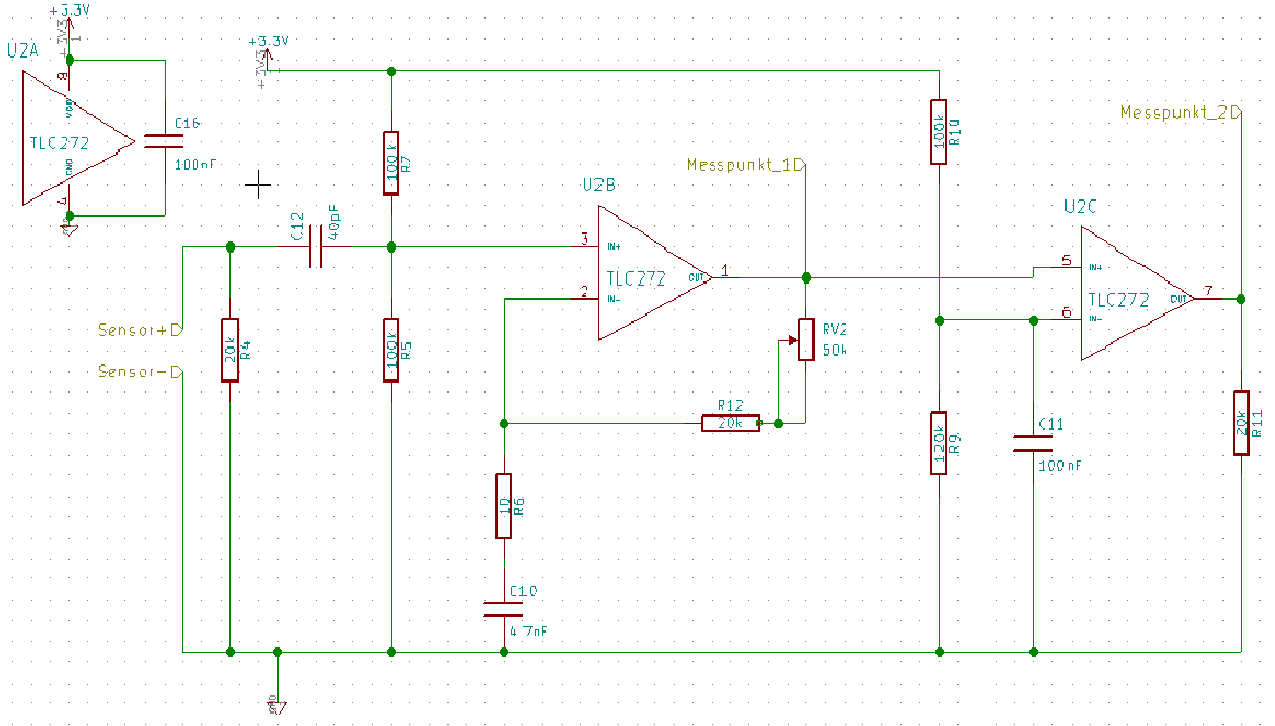
\includegraphics[width=1\textwidth%, draft
]{Abbildungen/Empfaenger.png}
\captionof{figure}{Schaltplan zweier Operationsverstärker mit einer vorgelagerten Filterung als Empfängerschaltung}
\label{fig:Empfaengerschaltung}
\end{minipage}\\
\end{center}


\section{Entwicklung der Software zum Betrieb des Prototypen}
\subsection{Benötigte Kenntnisse}
Um das Programm zu erstellen sollten Kenntnisse z.B. für die Capture Compare Unit des Mikrocontrollers vorhanden sein. Die CCU4 hat insgesamt 4 Einheiten und jede einzelne besitzt mehrer Slices von CC40 bis CC43. Slices können untereinander verschachtelt werden um so z.B. Interrupt Service Routinen aufzurufenird, siehe dazu das Reference Manuel.
Der Werte der Register mit denen die Zeit gemessen wird müssen sofort zum beginn der Interrupt Service Routine zwischengespeichert werden damit sichergestellt wird das nicht die Zeit zur Brechung mit gemessen wird.\\

\subsubsection{Durchgeführte Berechnungen}
Auch für die Programmierung waren diverse Berechnungen notwendig. Zur Erzeugung der Ultraschallimpulse wurde ein pulsweitenmoduliertes Rechtecksignal mit einer Frequenz von 40~kHz generiert. Dafür war es notwendig mit Hilfe der CCU4 einen Timer zur erstellen. So musste bei einem Timertakt von 96~MHz eine Periodendauer von 2400 Takten und einem Compare\_Wert von 1200 Takten  konfiguriert werden. Im Zählvorgang des Timers wird der Ausgang nach erreichen des Compare-Wertes auf 1 gesetzt, und nach erreichen der Periodendauer wieder auf 0 zurückgesetzt. Dadurch ergibt sich eine Periodendauer von 25~\textmu s, was einer Frequenz von 40~kHz entspricht.\\
Die Zeit die vergeht bis das Echo des Ultraschall-Impulses zurück kommt wird über einen Timer erfasst. 
\onehalfspacing \\ \\
\(\displaystyle Periodendauer=\frac{96~MHz}{40~kHz} = 2400 \),  \  \  \    \(\displaystyle Compare\_Wert=\frac{2400}{2} = 1200 \) 
\singlespacing


\subsection{Quellcodeentwurf}

\textbf{Programmstruktur:}\\
In der  Distance US main.c befinden sich nur Funktionsaufrufe die eine Grundkonfiguration  für den Controller beinhaltet und eine Schleife die immer wieder abgerufen wird um z.B. eine neue Entfernungsmessung zu starten, siehe Abbildung \ref{fig:main.c1}. Anstatt alles in der Distance US main.c an Programmcode zu verfassen was bei  komplexen Programmen schnell zu Unübersichtlichkeit führt hat das Auslagern den Vorteil das der Quellcode Logisch getrennt werden kann und einer verschlankerung des Codes mit sich bringt. 
Somit stehen in der Main  vor allem die Aufrufe der benötigten Funktionen. 
Auch vereinfacht diese Struktur gerade bei Prototypen das Testen der Funktion. So kann im Falle einer fehlerhaften Funktion einfach der Aufruf auskommentiert werden um zu testen, ob der Fehler wirklich von der Funktion herrührt. Dadurch müssen nicht etliche Zeilen Programmcode der Funktion auskommentiert werden, wodurch schnell Fehler entstehen könnten, durch übriggebliebene Zeichen, oder gar beim entfernen der Auskommentierung gelöschte Zeichen.\\
\begin{minipage}{1\textwidth}
\begin{lstlisting}
#include <stdio.h>
#include <stdbool.h>
#include "bricklib2/logging/logging.h"
#include "bricklib2/bootloader/bootloader.h"
#include "communication.h"
/****Eigene Include Dateien*******/
#include "configs/config.h"
#include "system_timer/system_timer.h"
#include "a16pt.h"
int main(void)
{ 
	logging_init(); 
	logd("Start Distance US V2 Bricklet/n/r");  	//For the Debugmodus
	communication_init(); 					//Function call
	a16pt_init(); 								//Function call	
	while(true)
	{
		a16pt_tick(); 						//Function call
		bootloader_tick(); 					//Function call
		communication_tick(); 				//Function call
		
	}
}
\end{lstlisting}
\captionof{figure}{Die main.c des Distance US}
\label{fig:main.c1}
\end{minipage}\\
Um die Funktionsaufrufe wie die a16pt\_init und die a16pt\_tick zu verstehen muss die Abbildung \ref{fig:a16pt.h}: Headerdatei der a16pt.h näher betrachtet werden.
In der der Datei werden die Funktionen definiert und deren Funktionsanweisung steht dann in der a16pt.c.\\
\begin{minipage}{1\textwidth}
\begin{lstlisting}
#ifndef A16PT_H
#define A16PT_H
#include <stdint.h>
void a16pt_init(void);				//Functional definition
void a16pt_tick(void); 			//Functional definition
uint16_t a16pt_get_distance(void); //Functional definition
#endif
\end{lstlisting}
\captionof{figure}{Headerdatei der a16pt.h}
\label{fig:a16pt.h}
\end{minipage}\\
\\
\textbf{Init Aufruf:}
Auch in der Abbildung \ref{fig:a16pt.c}: Ein Teilausschnitt von der a16pt.c mit den Konfiguration Funktionen werden in der void a16pt-init(void)  weitere Funktionsaufrufe wie z.B. die PWM oder der Externe Interrupt aufgerufen und konfiguriert.

\begin{minipage}{1\textwidth}
\begin{lstlisting}
void a16pt_init(void)
{

/*****************Externe_Interrupt*******************/

	eru_init(eru_port);

/************PWM_Init*****************************/

	XMC_CCU4_Init(CCU41, XMC_CCU4_SLICE_MCMS_ACTION_TRANSFER_PR_CR_PCMP);
	XMC_CCU4_StartPrescaler(CCU41);

	ccu4_pwm_init(pwm_port_0,cc40, period_1);	//P4_4
	ccu4_pwm_set_duty_cycle( cc40, compare_1);

	ccu4_pwm_init(pwm_port_1,cc42, period_0);	//P4_6
	ccu4_pwm_set_duty_cycle( cc42, compare_0);
.
.
.
.
\end{lstlisting}
\captionof{figure}{Ein Teilausschnitt von der a16pt.c mit den Konfiguration Funktionen }
\label{fig:a16pt.c}
\end{minipage}



\textbf{Interrupt Aufruf:}
In der Abbildung \ref{fig:a16pt.c1} :a16pt.c Interrupt Request, werden die für die Entfernungsmessung notwendigen Funktionen und die Interrupt Anweisungen, in dem Fall die IRQ21, abgearbeitet. Außerdem werden die Timer synchron abgeschaltet und aus experimentellen gründen wurde ein weiterer Impuls generiert um zu beobachten wie sich das Nachschwingen bei einer längeren Kurzschlusszeit an der Ultraschallkapsell verhält. Die IRQ wird auch als Interrupt Request bezeichnet und wird von der Hardware oder von der Software ausgelöst.
\\
\begin{minipage}{1\textwidth}
\begin{lstlisting}

/*************Interrupt_Funktionen****************/

void IRQ_Hdlr_21(void) // Compare Interrupt counter 10
{

	// Disable IRQs so we can't be interrupted
	__disable_irq();

	// Set CCU trigger to low, otherwise ccu counter is restarted
	XMC_SCU_SetCcuTriggerLow(XMC_SCU_CCU_TRIGGER_CCU41);

	// Stop slice 2
	XMC_CCU4_SLICE_StopClearTimer(CCU41_CC40);

	// For slice 1 we wait until PWM is run through (to get exactly 10 pwm peaks on P4_4 and P4_6)
	while(XMC_CCU4_SLICE_GetTimerValue(CCU41_CC42) > compare_1) {

		__NOP();
	}
	
	//New pin configuration
	const XMC_GPIO_CONFIG_t pin_out_config	= {
			.mode                = XMC_GPIO_MODE_OUTPUT_PUSH_PULL,
			.output_level        = XMC_GPIO_OUTPUT_LEVEL_HIGH,
		};

	 XMC_GPIO_Init(P4_6, &pin_out_config);
	//Creatw a high impulse
	for(s=0; s<50; s++)
		{
			__NOP();
		}
	// Stop slice 0
	XMC_CCU4_SLICE_StopClearTimer(CCU41_CC42);
	
	//Pin configuration back to the PWM-Mode
	const XMC_GPIO_CONFIG_t gpio_out_config1	= {
		.mode                = XMC_GPIO_MODE_OUTPUT_PUSH_PULL_ALT9,
		.input_hysteresis    = XMC_GPIO_INPUT_HYSTERESIS_STANDARD,
		.output_level        = XMC_GPIO_OUTPUT_LEVEL_LOW,
	};

	XMC_GPIO_Init(P4_6, &gpio_out_config1);
	// Enable IRQs again
	__enable_irq();


}
\end{lstlisting}
\captionof{figure}{Ein Teilausschnitt von der a16pt.c mit einem Interrupt Request}
\label{fig:a16pt.c1}
\end{minipage}

%\newpage
%\begin{minipage}{1\textwidth}Eventuell wo anders hin
%\begin{struktogramm}(120,75)
%\forever
%\assign{\#include aufrufe}
%\while[8]{int main (void)}
 %\sub{Logging init()}
 %\sub{logd ("start Distance us v2 Bricklet")}
 %\sub{Communication init()}
 %\sub{a16pt init()}
%\while[8]{while (1)}
 %\sub{a16pt\_tick()}
 %\sub{bootloader\_tick()}
% \sub{Communication\_tick()}
%\whileend
%\whileend
%\foreverend

%  \ifthenelse{10}{4}{Bedingung 1}{ja}{nein}
%    \ifthenelse{6}{6}{Bedingung 2}{ja}{nein}
%      \assign{Anweisungsblock 1}
%    \change
%      \assign{Anweisungsblock 2}
%    \ifend
%  \change
%    \assign{Anweisungsblock 3}
%  \ifend
%\sub{bla}
%\end{struktogramm}
%\captionof{figure}{Struktogramm der main}\label{fig:Struktogramm der main}
%\end{minipage}

%\newpage
%\begin{figure}[H]
%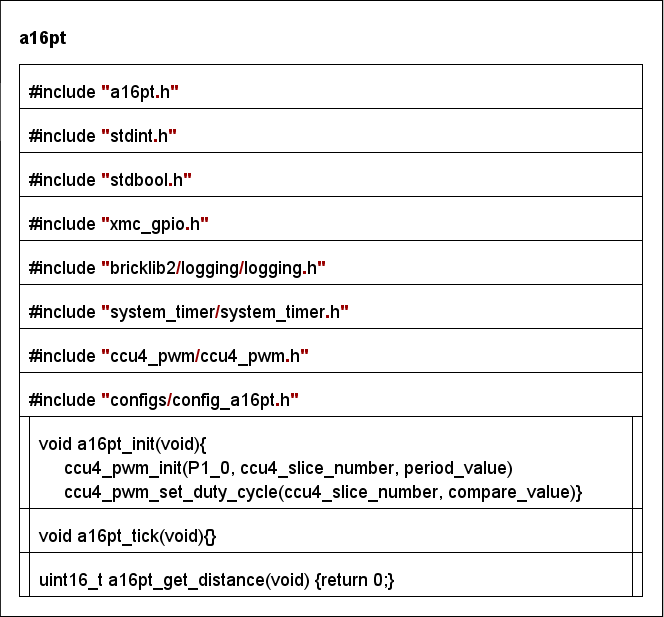
\includegraphics[width=1.0\textwidth]{Struktogramme/a16pt.png}\caption{Struktogramm der a16.pt}\label{fig:Bild2}
%\end{figure}




\chapter{Messungen und Auswertung der Ergebnisse}
\label{Messungen}
Für die Messungen wurden im Laufe des Projekts zwei Versionen an Prototyp-Platinen entworfen. Im Verlauf der Versuche wurden Veränderungen an den Platinen vorgenommen, um den Betrieb dieser zu verbessern. 
\section{Prototyp 1}
\begin{center}
\begin{minipage}{0.75\textwidth}
\includegraphics[width=1\textwidth%, draft
]{Abbildungen/BilderPrototypen/Prototyp1.JPG}
\captionof{figure}{Aufgebaute und bearbeitete Platine des ersten Prototypen}
\label{fig:Prototyp1}
\end{minipage}
\end{center}
Bei dem ersten Prototyp wurden die Sendereinheit und die Empfängereinheit auf getrennten Platinen aufgebaut. So bestand die Möglichkeit, den Senderkreis und den Empfängerkreis getrennt zu untersuchen, ohne dass elektrische Signale der beiden Schaltkreise überlagern konnten. Anfangs wurde für den Senderkreis eine komplette H-Brücke als Schalter verwendet. Allerdings war der Aufbau nicht funktional, da ein Beschaltungsfehler vorhanden war. Dieser wurde mit Fädeldraht provisorisch behoben.  Dadurch, dass das A5950 eine H-Brücke mit integrierter Kontroll-Logik und eigener Spannungspumpe ist, wurde anhand der Schaltweise der Baugruppe festgestellt, dass diese H-Brücke nicht für die Schaltung einsetzbar ist. Um nicht sofort eine neue Platine in Auftrag geben zu müssen, was einiges an Zeit gekostet hätte, wurde das IC ausgelötet. Danach wurde ein MOSFET als HIGH-Side an der Stelle eingesetzt. Dadurch ließen sich erste Versuche durchführen, nichtsdestotrotz entsprach das Ergebnis noch nicht den Anforderungen. Deswegen wurde die Beschaltung an dieser Stelle auf eine Halbbrücke erweitert. Damit war die Funktion des Senderkreises für die ersten Versuche und Messungen gegeben.\\
Der Empfängerkreis war von Beginn an funktional, konnte aber erst mit Inbetriebnahme des Senderkreises richtig getestet werden. Am Empfängerkreis wurden zu Testzwecken Änderungen an der Filterung, vor dem Verstärker, vorgenommen. Die Filterung wurde in ihrer Dimensionierung verändert, um herauszufinden, wie sich die Qualität des Echo-Signals verbessern lässt.\\

\subsection{Senderkreis}
Zuerst wurden Signale direkt an dem Mikrocontroller gemessen, um sicher zu stellen, dass die Einstellungen im Programm die gewünschten Ausgaben zur Folge haben, und keine Gefährdung der Bauteile entsteht.
Um das Signal für die Entfernungsmessung zu generieren wurde der Prozessor so programmiert, dass zehn Impulse mit einer Frequenz von 40~kHz ausgegeben werden. Danach erfolgt eine Pause, um das zurückkehrende Signal abzuwarten und auszuwerten.\\
\begin{minipage}{0.46\textwidth}
\includegraphics[width=1\textwidth%, draft
]{Abbildungen/MessungenP1/PWM-von-der-cpu.png}
\captionof{figure}{PWM-Burst auf 40~kHz Basis an der CPU}
\label{fig:pwm-burst}
\end{minipage}\qquad
\begin{minipage}{0.46\textwidth}
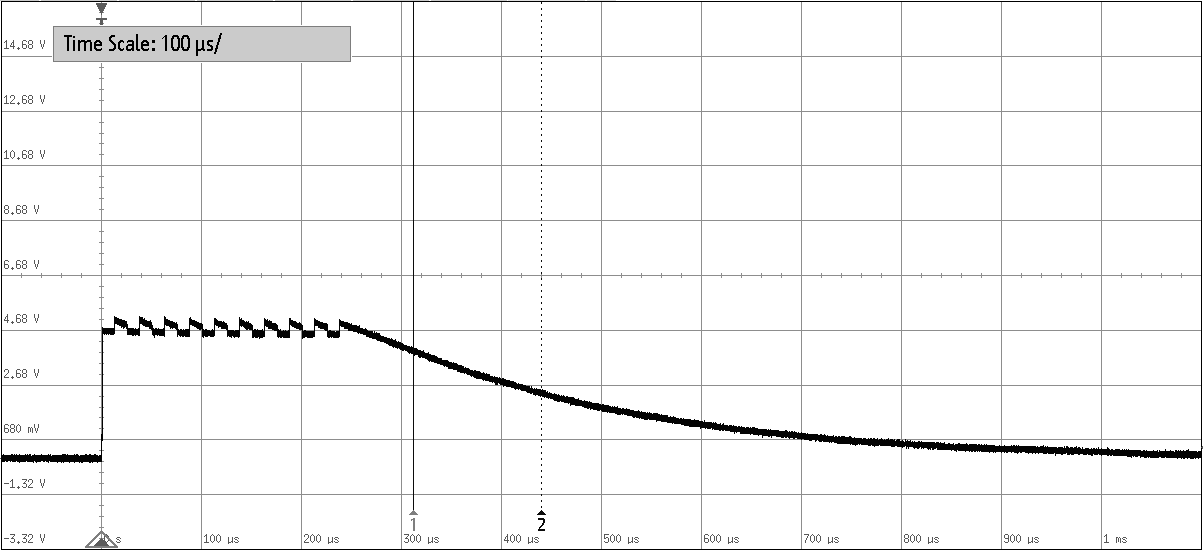
\includegraphics[width=1\textwidth%, draft
]{Abbildungen/MessungenP1/PWM-ausgabe-mit-Hi-Side.png}
\captionof{figure}{PWM Ausgabe über einen HIGH-Side}
\label{fig:HiSide}
\end{minipage}\\
In der Abbildung \ref{fig:pwm-burst} ist zu sehen, dass der gewünschte Burst aus zehn Impulsen mit einer Periodendauer von jeweils 25~\textmu s vom Mikrocontroller generiert wurde. Diese Messung wurde auch vorgenommen, um zu überprüfen, wie das Signal durch die eingesetzten Bauteile verändert wird.\\
Die Abbildung \ref{fig:HiSide} zeigt, wie das Ausgangssignal nach einer HIGH-Side aussieht. So wird zwar im Takt des PWM-Signals geschaltet, allerdings fehlt es an einem Gegenpol, um das Potential in den Schaltpausen wieder auf Null zu ziehen. Dadurch bleibt die Spannung während des Schaltens immer auf einem erhöhten Pegel und sinkt erst nach Ende des PWM-Signals allmählich ab. Dadurch kann keine vernünftige Ausgabe an der Ultraschallkapsel erzeugt werden, denn ohne deutliche Potentialunterschiede kann dieser auch nicht in Schwingungen versetzt werden. Der ausgegebene Schalldruck würde nur für kurze Entfernungsmessungen reichen. Das zurückkommende Signal wird von der abklingenden Spannung des HIGH-Side überlagert. Somit ist dieser Aufbau nicht umsetzbar.\\
Um die Spannung nicht nur auf einen HIGH-Pegel, sondern auch auf einen LOW-Pegel schalten zu können wurde danach auf eine Halbbrücke gewechselt. Mit dieser lässt sich der Ausgang, über zwei durch das PWM-Signal gesteuerte MOSFETs, sauber auf HIGH- oder LOW-Pegel schalten. 
Mit der verwendeten Halbbrücke ergab sich die Abbildung \ref{fig:Halfbridge}\\
\begin{minipage}{0.46\textwidth}
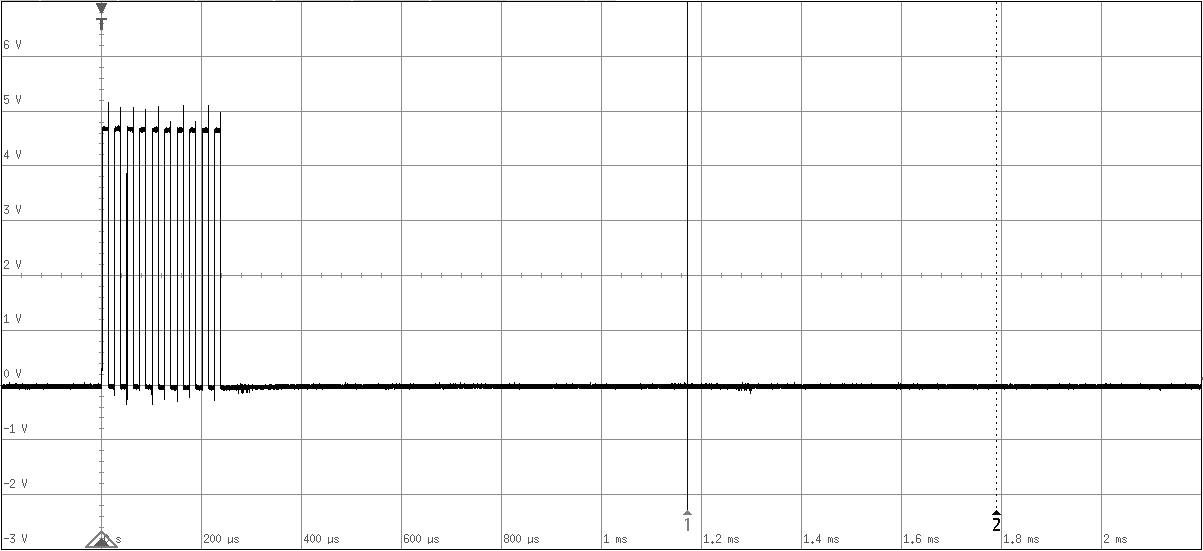
\includegraphics[width=1\textwidth%, draft
]{Abbildungen/MessungenP1/PWM-Nach-der-Halbbrucke.png}
\captionof{figure}{PWM Ausgabe über eine Halbbrucke}
\label{fig:Halfbridge}
\end{minipage}\qquad
\begin{minipage}{0.46\textwidth}
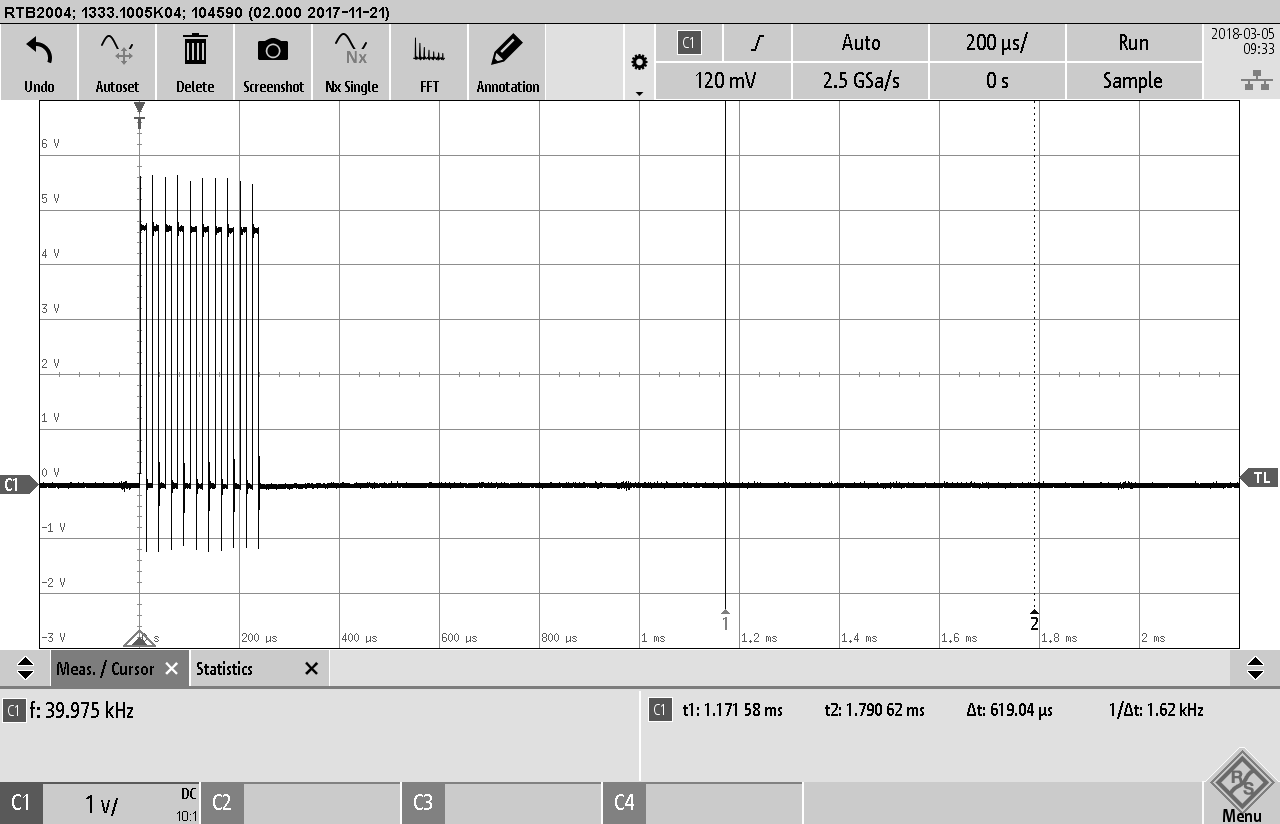
\includegraphics[width=1\textwidth%, draft
]{Abbildungen/MessungenP1/PWM-Nach-der-Halbbrucke-mit-LS.png}
\captionof{figure}{Ausgabe der PWM an der Ultraschallkapsel}
\label{fig:Senderausgabe}
\end{minipage}\\
Es zeigt sich, dass das Signal nach der Erweiterung auf eine Halbbrücke wieder wie das von dem Mikrocontroller ausgegebene PWM-Signal aussieht. Vergleiche Abbildung \ref{fig:pwm-burst}. Die Amplitude fällt wie geplant höher aus. Somit kann die Höhe der Amplitude über die Spannungspumpe variiert werden um die Stärke des ausgegebenen Signals zu verändern, ohne den Mikrocontroller durch die höhere Spannung zu beschädigen. Wie in der Abbildung \ref{fig:Senderausgabe} zu entnehmen ist, entstehen durch die angeschlossene Ultraschallkapsel höhere Spannungsimpulse in den Schaltmomenten. Diese Spannungsspitzen, die durch die Ultraschallkapsel entstehen, wurden in den Expirementen vernachlässigt, da keine Gefährdung anderer Bauteile entstand. Das somit generierte Ausgangssignal entsprach den Anforderungen und musste für die Versuche nicht weiter bearbeitet werden.
\subsection{Empfängerkreis}
Die Platinen des Sender- und Empfängerkreises wurden gemeinsam auf einer Halterung montiert, dass die Ultraschallkapseln zum senden und empfangen der Signale nebeneinander befestigt werden konnten. Ziel war es, durch verschieben eines Hindernisses die Signaländerungen an den Platinen beobachten zu können, ohne die gesamten Messaufbauten bewegen zu müssen. Bei der Aufnahme der Messungen wurde der Empfängerkreis Schritt für Schritt überprüft, um zu erfahren, wie sich das empfangene Signal durch die einzelnen Bauteile verändert.\\
\begin{minipage}{0.46\textwidth}
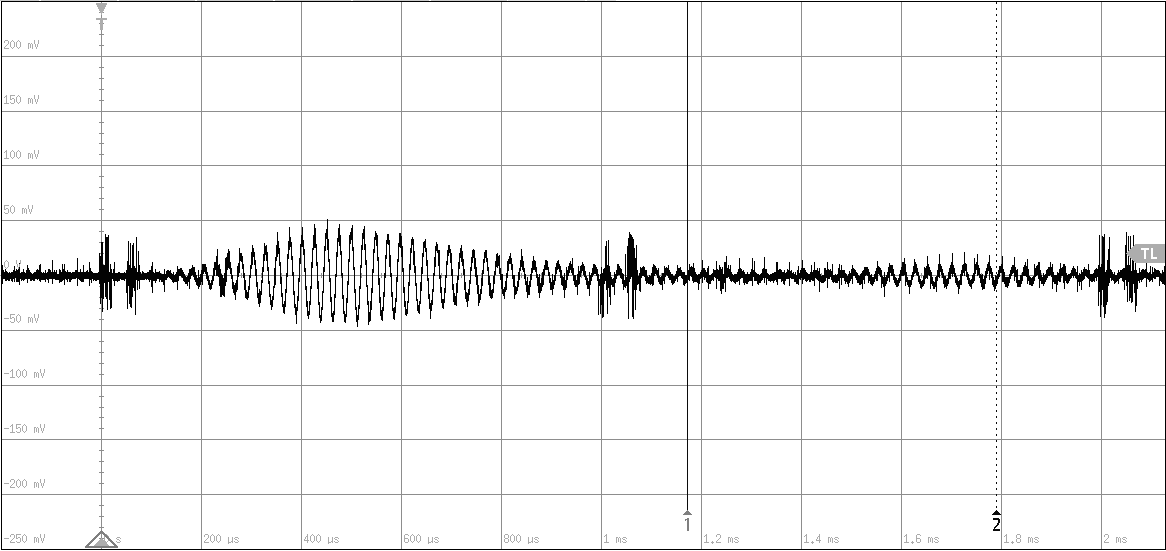
\includegraphics[width=1\textwidth%, draft
]{Abbildungen/MessungenP1/Signal-Empfang.png}
\captionof{figure}{Signal Empfang}
\label{fig:Empfang am LS}
\end{minipage}\qquad
\begin{minipage}{0.46\textwidth}
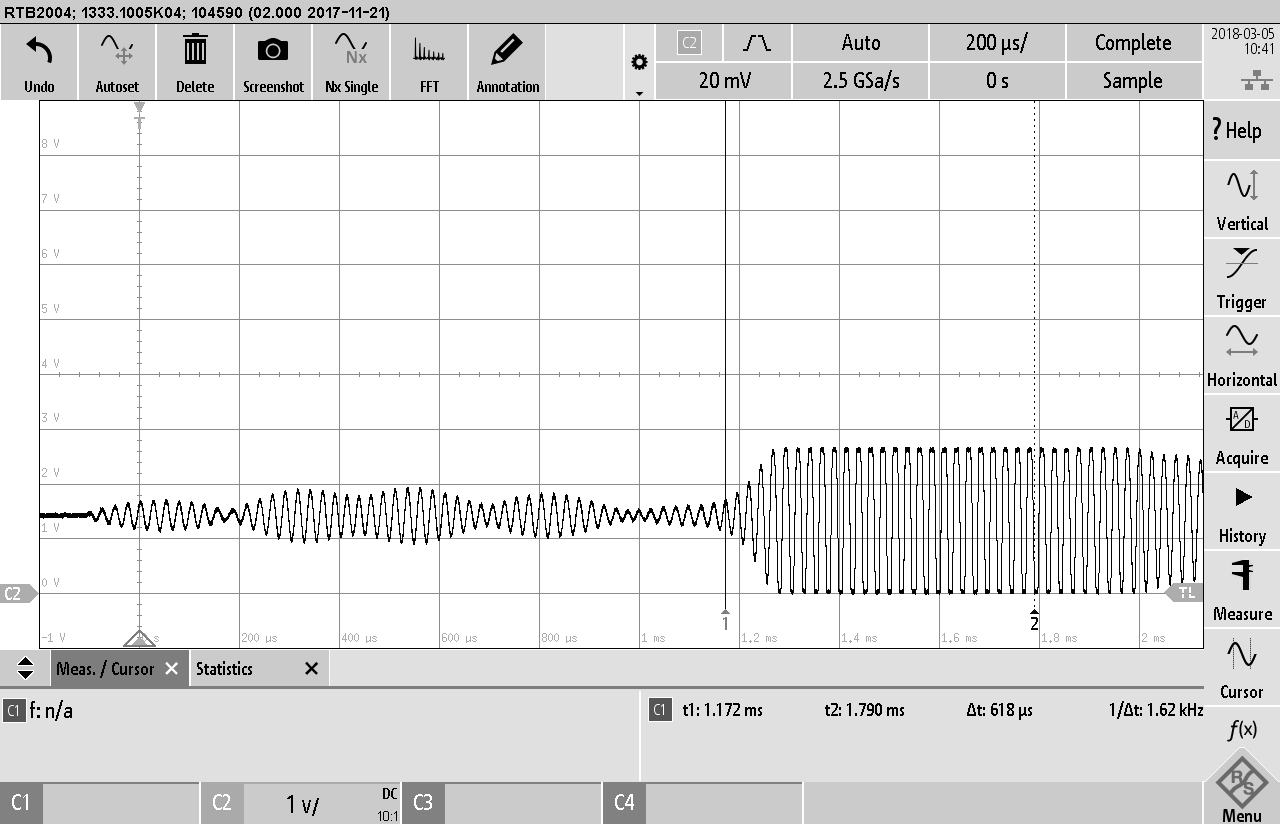
\includegraphics[width=1\textwidth%, draft
]{Abbildungen/MessungenP1/Signal-nach-Verstarkung.png}
\captionof{figure}{Signal nach Verstärkung}
\label{fig:Verstaerkung}
\end{minipage}\\
Die Abbildung \ref{fig:Empfang am LS} zeigt das Signal, das direkt am Empfänger zu messen war. Hier sind verschiedene vorerst nicht zuordenbare Signale zu sehen. Allein aus diesem Bild lässt sich daher keine Aussage zu den einzelnen Signalen machen. Fest steht nur, dass ebenfalls Signale die nicht der gewünschten Frequenz entsprechen, vom Empfänger aufgenommen werden. Dieses Problem gilt es natürlich zu beheben, um unerwünschte Störungen zu vermeiden.
Die Abbildungen \ref{fig:Verstaerkung} und \ref{fig:Verstaerkung2} zeigen den Verlauf des Signals nach der Filterung und Verstärkung in zwei verschiedenen Zeitauflösungen. Dabei entspricht \ref{fig:Verstaerkung} den ersten drei Messintervallen von \ref{fig:Verstaerkung2} und dient um darzustellen, dass die Verstärkung eine maximale Aussteuerung von 3,3~V nicht überschreitet.\\
\begin{minipage}{0.46\textwidth}
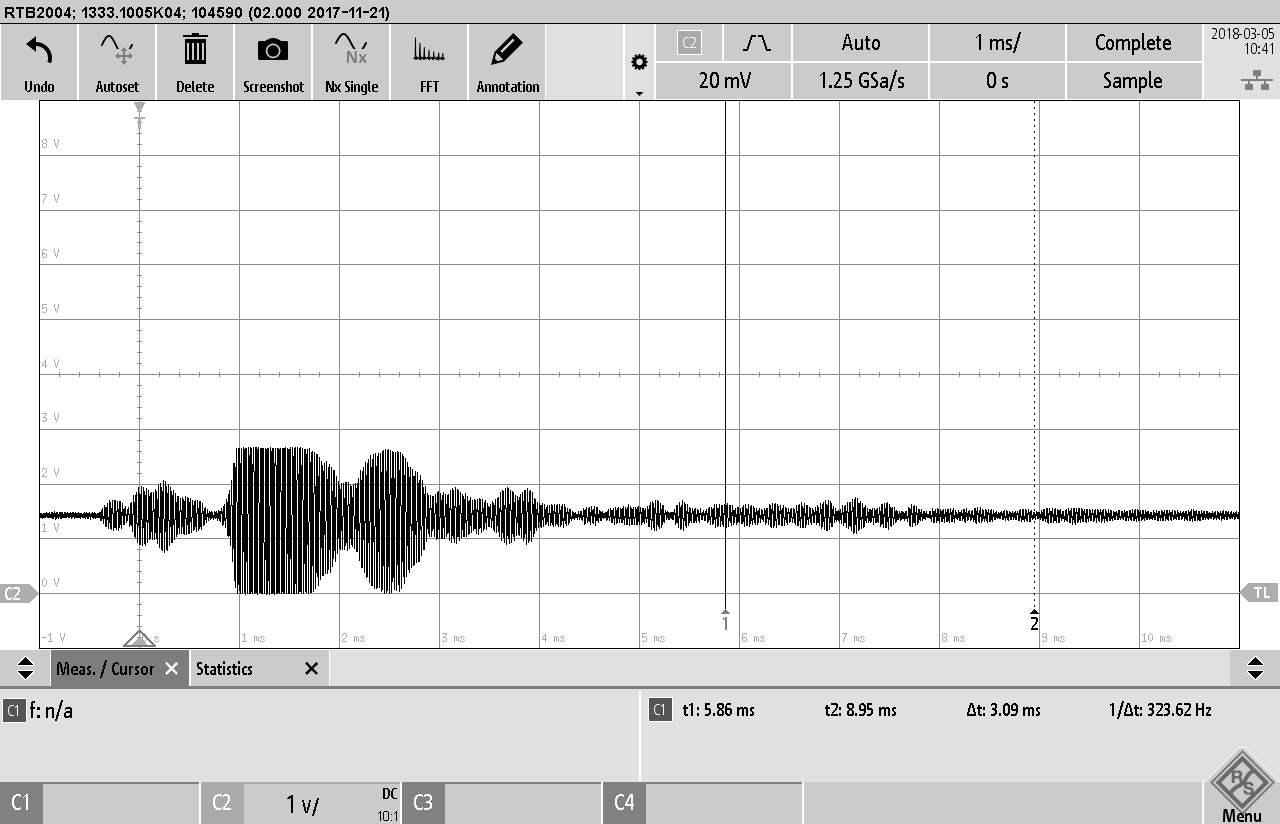
\includegraphics[width=1\textwidth%, draft
]{Abbildungen/MessungenP1/Signal-nach-Verstarkung2.png}
\captionof{figure}{Signal nach Verstärkung 2}
\label{fig:Verstaerkung2}
\end{minipage}\qquad
\begin{minipage}{0.46\textwidth}
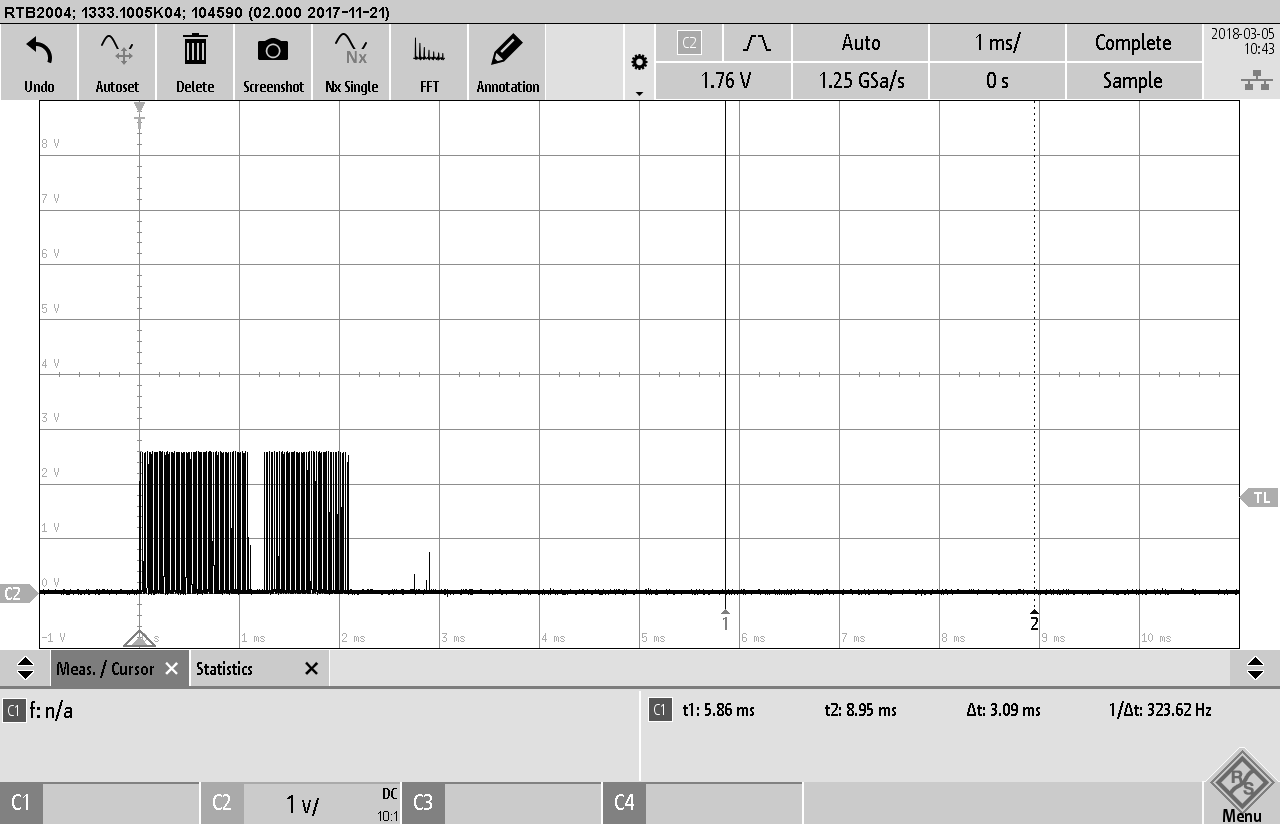
\includegraphics[width=1\textwidth%, draft
]{Abbildungen/MessungenP1/Signal-nach-Komparator.png}
\captionof{figure}{Signal nach Komparator}
\label{fig:Komparator}
\end{minipage}\\
Nach dem das Signal den Komparator passiert hat, ergibt sich das Bild wie in Abbildung \ref{fig:Komparator} zu sehen ist. Bei einem Vergleich mit dem Signal nach der Verstärkung \ref{fig:Verstaerkung2} wird sichtbar, dass der Komparator nur Signale, die über seinem Schwellwert von 1,8~V liegen, durchschaltet. Die Aufteilung in zwei Signalblöcke in den Abbildungen kommt daher, dass der erste Block das Signal der Sender-Kapsel ist, das direkt beim Senden seitlich auf die Empfänger-Kapsel abgestrahlt wurde. Der zweite Block ist bereits das Echo, das vom 20~cm entfernten Hindernis zurückgeworfen wurde.\\
Auch wurden Vergleichsmessungen mit Ultraschallkapseln verschiedener Hersteller durchgeführt. Für die nachfolgenden Abbildungen wurden  Ultraschallkapseln des Herstellers MURATA verwendet. Für Abbildung \ref{fig:MURATAs1,5m} wurden sowohl für den Sendebetrieb, als auch für den Empfängerbetrieb als Sender deklarierte Ultraschallkapseln verwendet. Für die Abbildung \ref{fig:MURATAsr1,5m} wurden die Kapseln entsprechend der Beschriftung verwendet.\\
\begin{minipage}{0.46\textwidth}
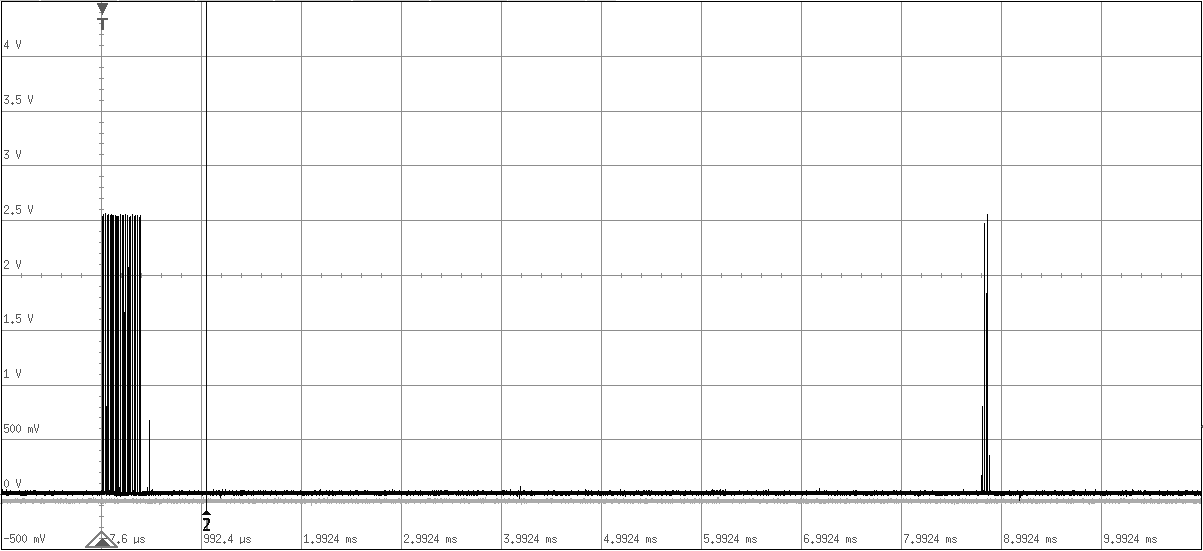
\includegraphics[width=1\textwidth%, draft
]{Abbildungen/MessungenP1/MURATAs1,5m.png}
\captionof{figure}{}
\label{fig:MURATAs1,5m}
\end{minipage}\qquad
\begin{minipage}{0.46\textwidth}
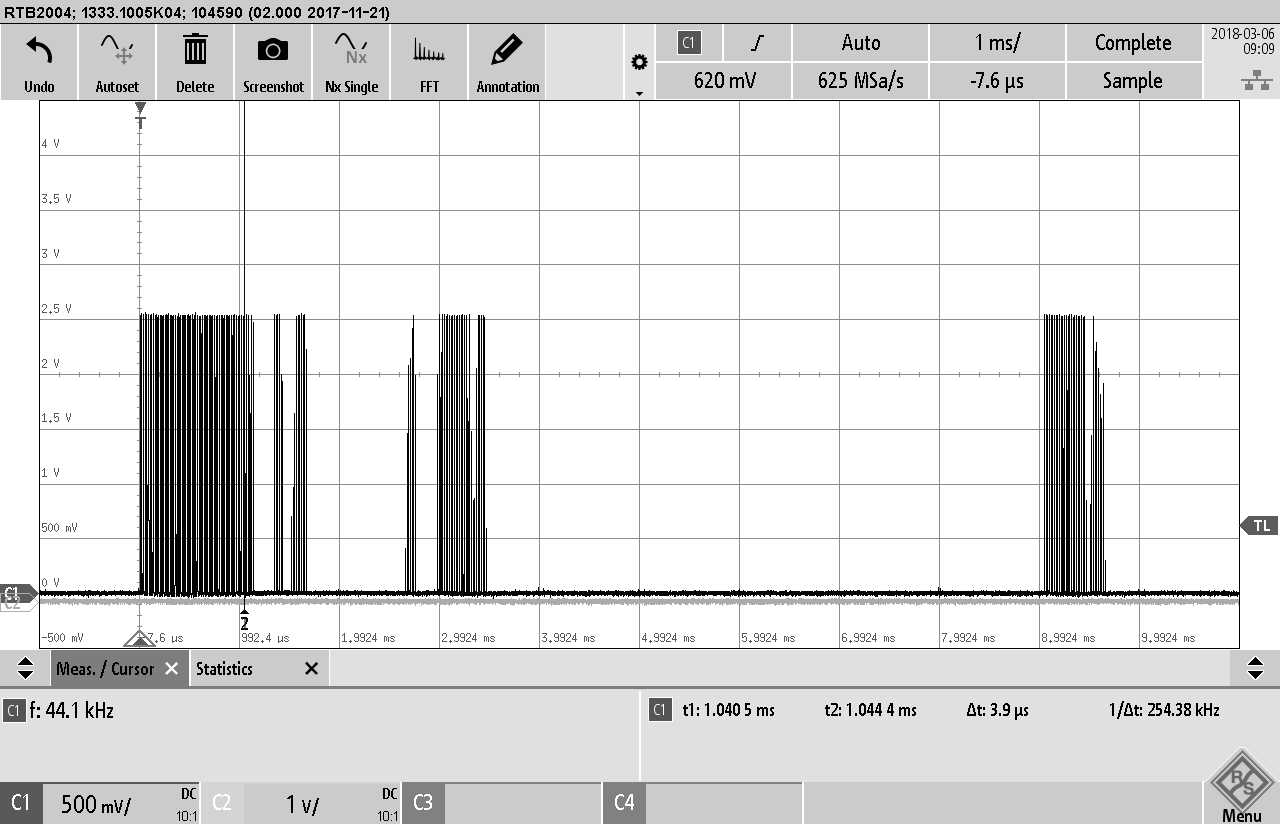
\includegraphics[width=1\textwidth%, draft
]{Abbildungen/MessungenP1/MURATAsr1,5m.png}
\captionof{figure}{}
\label{fig:MURATAsr1,5m}
\end{minipage}\\
Bei Betrachtung der beiden Abbildungen ist zu sehen, dass bei beiden Varianten zwar Signale empfangen werden. Bei Aufnahme der Abbildung \ref{fig:MURATAs1,5m} war die Empfindlichkeit des Empfängers wesentlich geringer als bei Abbildung \ref{fig:MURATAsr1,5m}. Daraus ergibt sich, dass bei diesem Hersteller die Sender- und die Empfängerkapsel bauliche Unterschiede aufweisen. Aus weiteren Vergleichsmessungen ging hervor, dass die Ultraschallkapseln des Herstellers EKULIT weder vertauscht, noch verpolt werden können. Bei allen Versuchen blieben die Resultate immer gleich. Demnach gibt es keinen baulichen Unterschiede bei den Sender- und Empfängerkapseln dieses Herstellers.
Anhand der gesammelten Ergebnisse kann festgehalten werden, dass die einfachere Version des Ultraschall-Entfernungsmessers durchaus simpel umzusetzen ist. Es fehlt nur noch ein Programm, das die Zeit zum Eintreffen des Echo-Signals in einen Abstand zum Hindernis konvertiert. Besagtes Programm wurde nicht für diese Prototyp-Version erstellt, da der Anspruch bestand, den Betrieb nicht nur über eine Platine, sondern noch über eine Ultraschallkapsel ablaufen zu lassen.
\newpage
\section{Prototyp 2}
\begin{center}
\begin{minipage}{0.75\textwidth}
\includegraphics[width=1\textwidth%, draft
]{Abbildungen/BilderPrototypen/Prototyp2.JPG}
\captionof{figure}{Aufgebaute und bearbeitete Platine des zweiten Prototypen}
\label{fig:Prototyp2}
\end{minipage}
\end{center}
Nachdem mit der ersten Prototyp-Version Versuche an der Elektronik durchgeführt wurden und erste Messungen mit einem beweglichen Hindernis auswertbare Ergebnisse brachten, wurde eine zweite Prototyp-Version entworfen. Bei der zweiten Prototyp-Version wurden der Sender- und der Empfängerkreis auf einer Platine aufgebaut und es wurde nur noch eine Ultraschallkapsel für beide Anwendungen vorgesehen. Dadurch wurden für den fehlerfreien Betrieb drei und nicht zwei Schaltzustände der Halbbrücke benötigt. Deswegen wurde die Halbbrücke der ersten Prototyp-Version durch eine voll gesteuerte Halbbrücke ersetzt. Nicht nur sollte die Ultraschallkapsel mit HIGH-, oder LOW-Signal steuerbar sein, auch ein dritter potentialfreier Zustand war nötig, damit die Echo-Signale auch empfangen werden konnten. Um bei diesem Aufbau einen fehlerfreien Betrieb der verwendeten voll gesteuerten Halbbrücke sicherzustellen wurden durch den Mikrocontroller zwei ineinander verschachtelte PWM-Signale generiert. Diese sind wie in der Abbildung \ref{fig:PWMs} zu sehen ist durch eine Lücken getrennt. Verzögerungen im Schaltbetrieb der Halbleiter konnten daher, keine Kurzschlüsse mehr verursachen. Dazu konnten durch den neuen Platinenentwurf die ab der ersten Prototyp-Version vorgenommenen Änderungen direkt in den Schaltplan übernommen werden. Dadurch ließ sich die Störanfälligkeit durch empfindliche Drahtbrücken deutlich reduzieren. Bedingt durch anfängliche Befürchtungen wurden für die MOSFETs der Halbbrücke anfangs jeweils ein weiteres MOSFET vorgeschaltet. Dieser Zusatz stellte sich als unnötig heraus, da durch eines der zusätzlichen Bauteile eines der PWM-Signale invertiert wurde. Somit wurde das überflüssige MOSFET entfernt. Durch zwei Drahtbrücken konnte die komplette Schaltung nach Behebung eines weiteren Verdrahtungsfehlers, in Betrieb genommen werden.\\
\begin{center}
\begin{minipage}{0.75\textwidth}
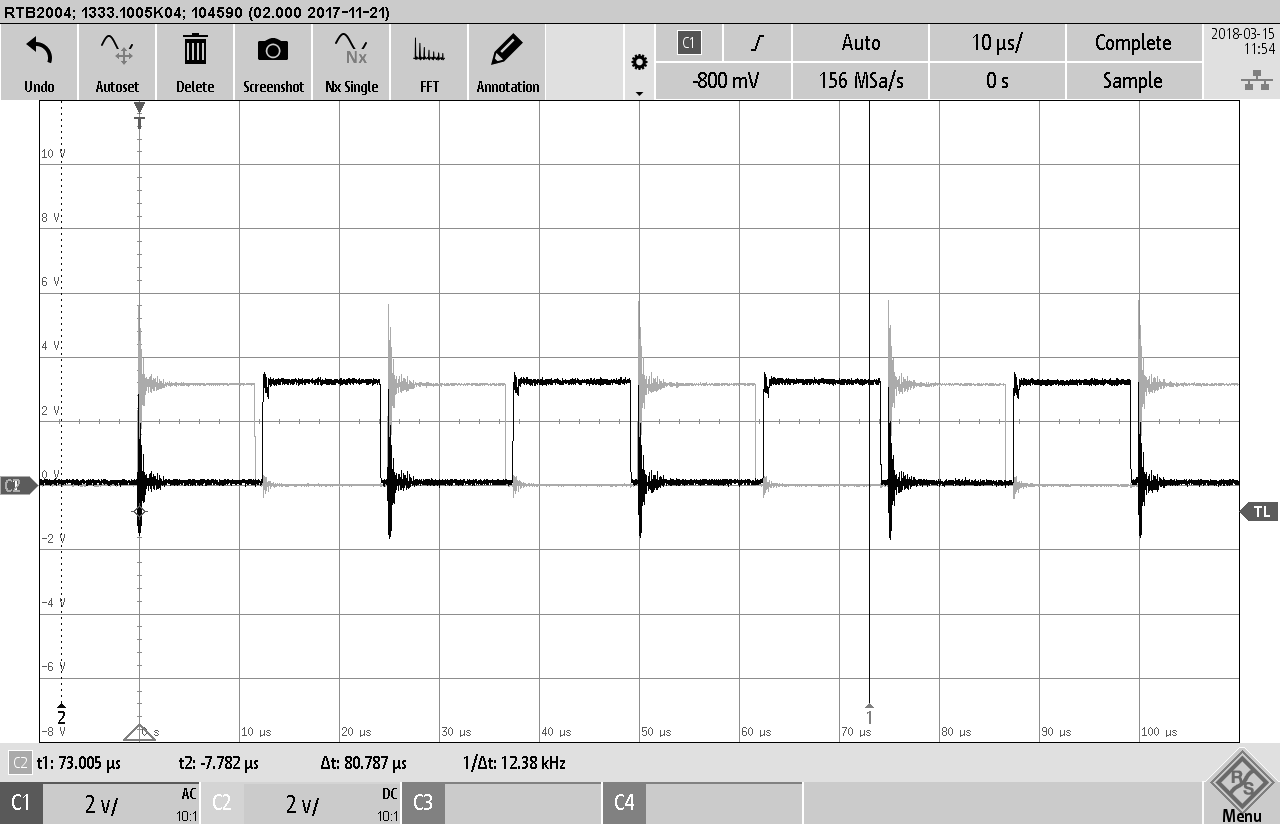
\includegraphics[width=1\textwidth%, draft
]{Abbildungen/MessungenP2/Zwei_PWMs_von_der_CPU.PNG}
\captionof{figure}{Verlauf der zwei generierten PWMs für den Betrieb der voll gesteuerte Halbbrücke}
\label{fig:PWMs}
\end{minipage}\\
\end{center}
Nachdem dieser Betrieb sichergestellt war, wurden Messungen am Verstärker (obere Linie), und am Komparator (untere Linie) vorgenommen. Dabei wurde die Verstärkung so eingestellt, dass unerwünschte Störungen nicht vom Komparator weitergegeben wurden. Die Spannung für den Sendebetrieb wurde für die Versuche zwischen 5\,V und 20\,V variiert, um betrachten zu können, wie sich das auf die Reichweite und Genauigkeit der Messungen auswirkt. Als Hindernis wurde bei allen Experimenten eine glatte Holzplatte der Maße 50x64\,cm verwendet und in einem Abstand von ein bis fünf Metern von der Ultraschallkapsel entfernt aufgestellt. In den Abbildungen \ref{fig:5v1m} bis \ref{fig:5v4m} sind die Ergebnisse einer Messreihe mit einer Spannung von 5\,V für den Sendebetrieb dargestellt. Die Ansicht wurde so eingestellt, dass zwei Sendeimpulse zu sehen sind. Dadurch wird deutlicher, welches die Sende Impulse sind, und welches die von der Entfernung abhängigen Echos sind.\\
\begin{minipage}{0.46\textwidth}
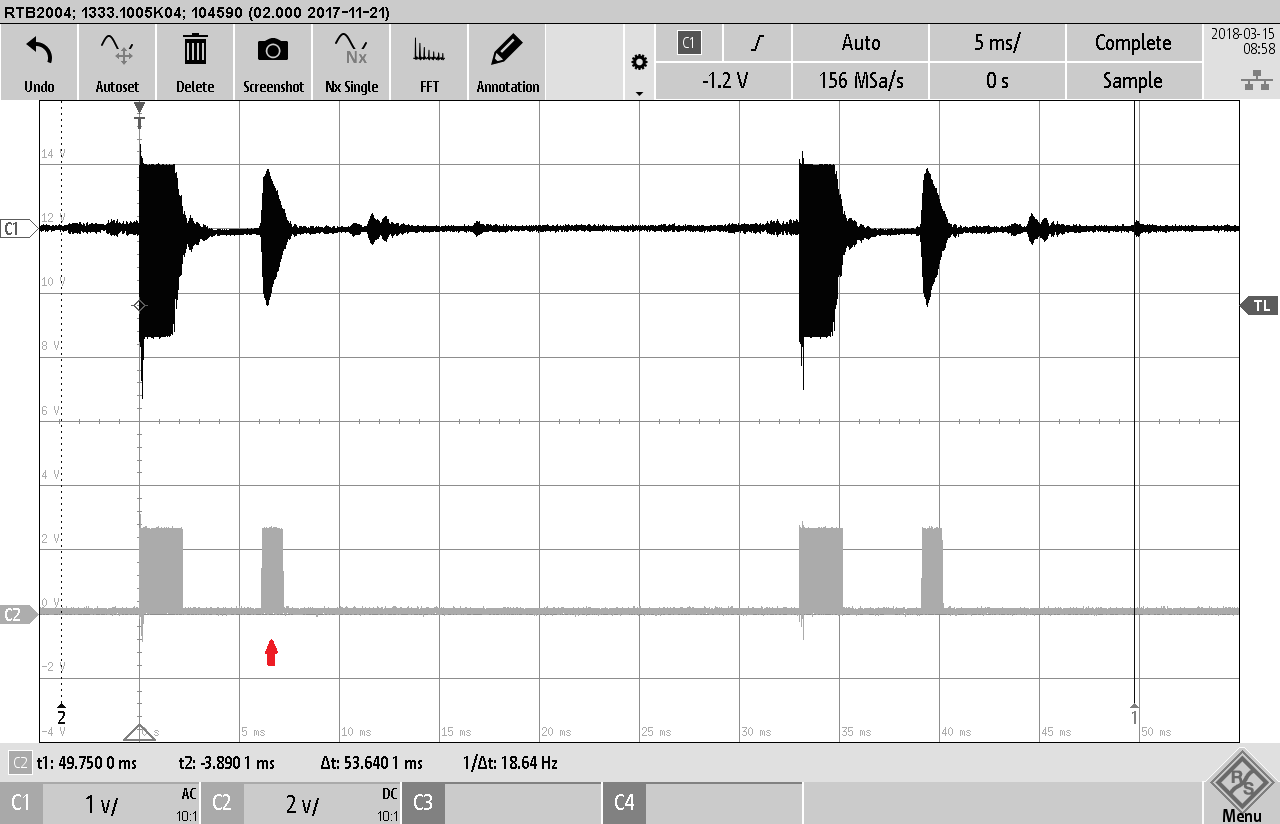
\includegraphics[width=1\textwidth%, draft
]{Abbildungen/MessungenP2/5V/1mb.PNG}
\captionof{figure}{Signalverlauf bei 5~V auf 1~m Abstand}
\label{fig:5v1m}
\end{minipage}\qquad
\begin{minipage}{0.46\textwidth}
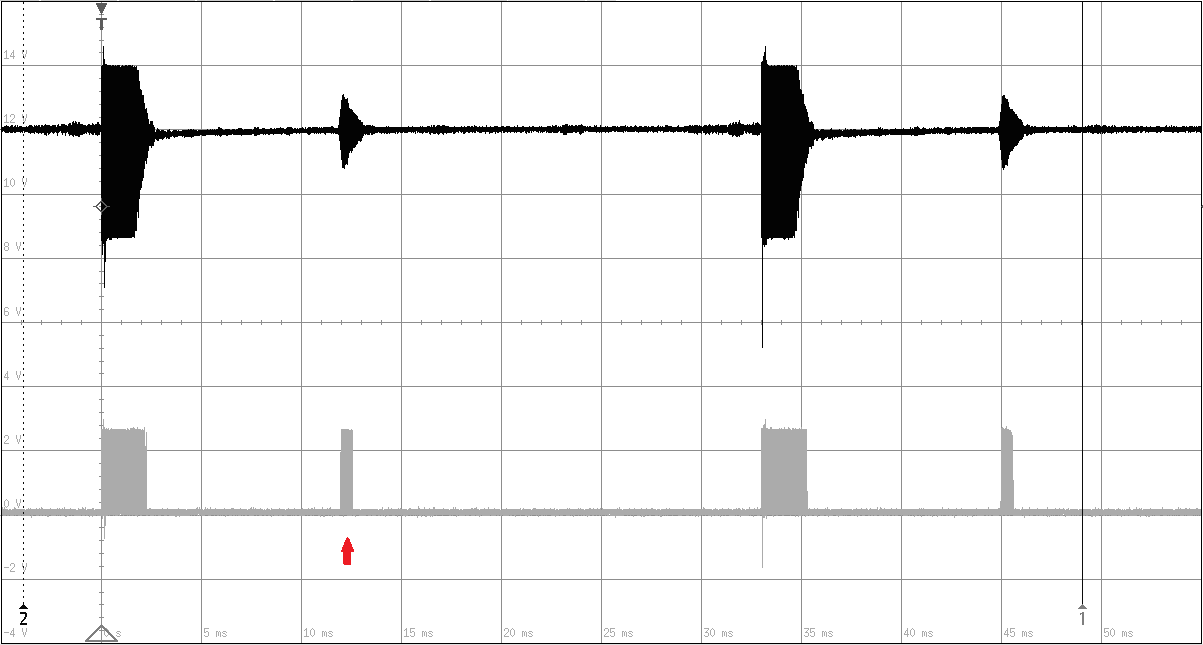
\includegraphics[width=1\textwidth%, draft
]{Abbildungen/MessungenP2/5V/2mb.PNG}
\captionof{figure}{Signalverlauf bei 5~V auf 2~m Abstand}
\label{fig:5v2m}
\end{minipage}\\
\begin{minipage}{0.46\textwidth}
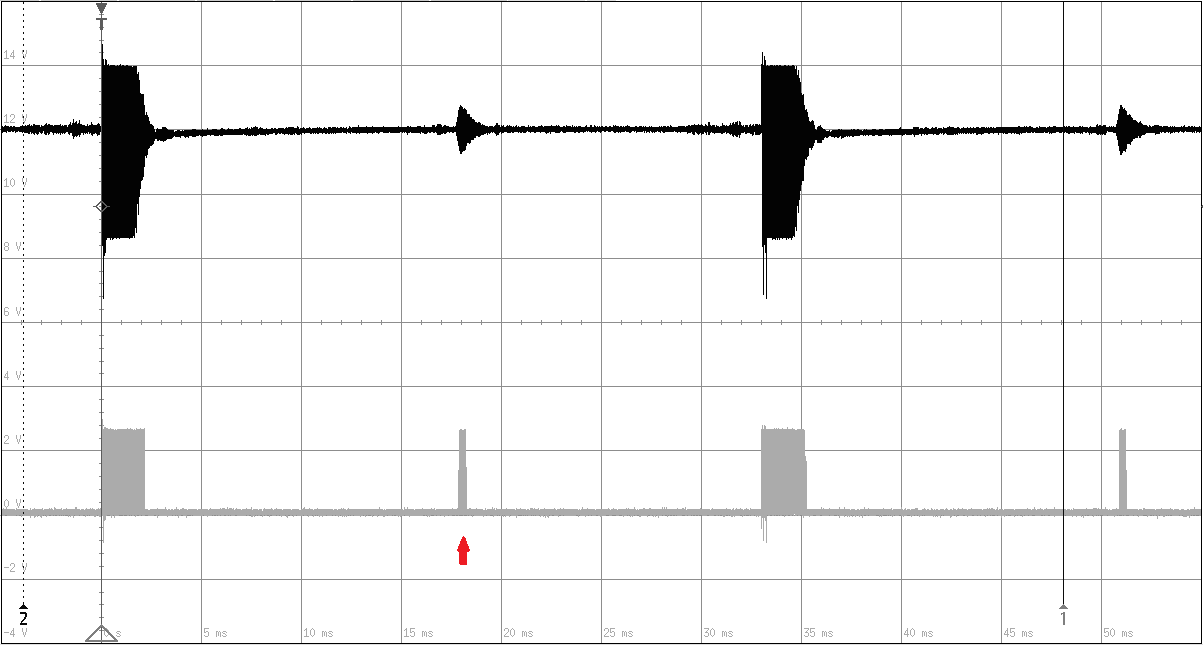
\includegraphics[width=1\textwidth%, draft
]{Abbildungen/MessungenP2/5V/3mb.PNG}
\captionof{figure}{Signalverlauf bei 5~V auf 3~m Abstand}
\label{fig:5v3m}
\end{minipage}\qquad
\begin{minipage}{0.46\textwidth}
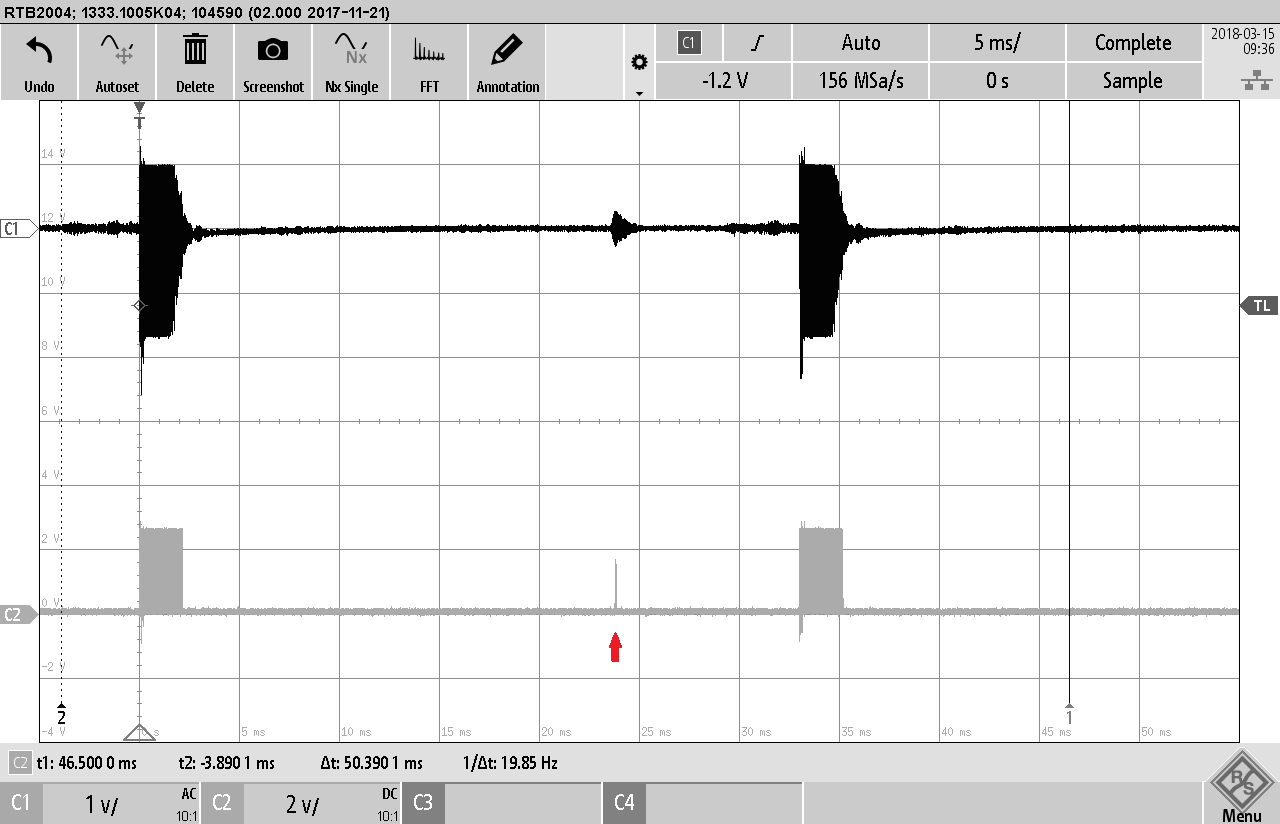
\includegraphics[width=1\textwidth%, draft
]{Abbildungen/MessungenP2/5V/4mb.PNG}
\captionof{figure}{Signalverlauf bei 5~V auf 4~m Abstand}
\label{fig:5v4m}
\end{minipage}\\
Bei den Abbildungen ist zu sehen, dass das Echo-Signal mit zunehmender Entfernung immer schwächer wird. Bei einer Entfernung von vier Metern (Abbildung \ref{fig:5v4m}) wird das Echo-Signal so schwach, dass die Signalstärke nach dem Komparator nicht mehr für eine eindeutige Auswertung über den Mikrocontroller ausreicht. Nachfolgend sind die Abbildungen einer Messreihe mit verschiedenen Spannungseinstellungen für den Sendebetrieb zu sehen. Anhand dieser Messreihe soll dargestellt werden, welchen Einfluss die eingestellte Spannung im Sendebetrieb auf die Reichweite des Ultraschallsignals hat. Für die Darstellung wurden die Messungen bei 5 Meter Abstand ausgewählt.\\
\begin{minipage}{0.46\textwidth}
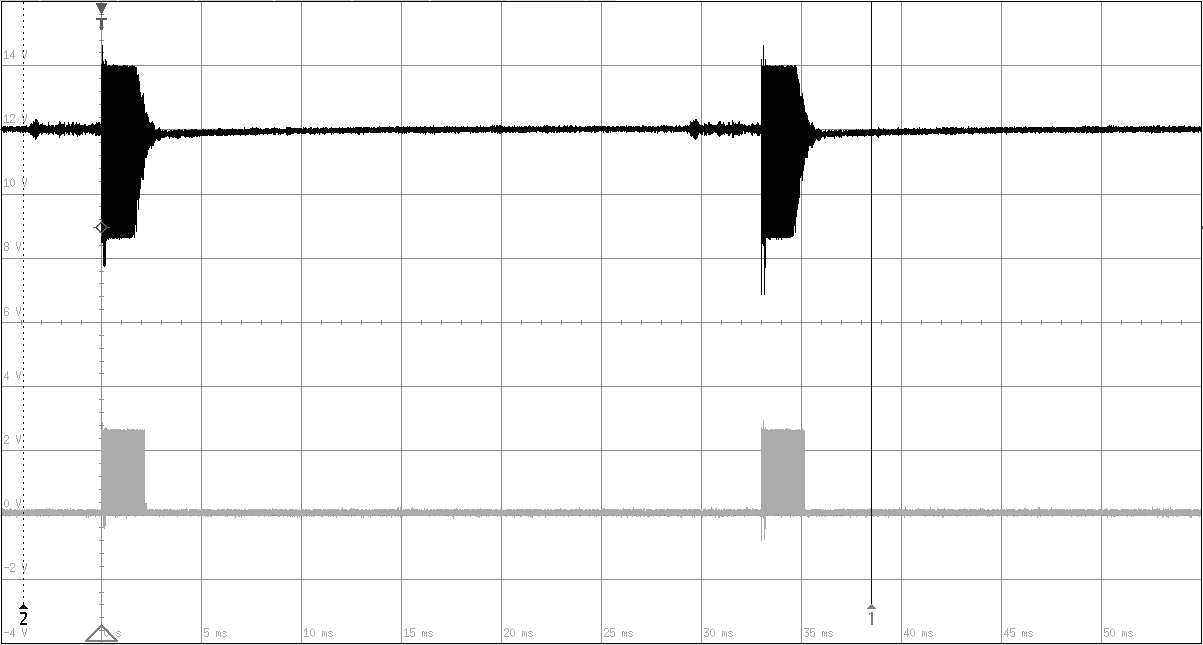
\includegraphics[width=1\textwidth%, draft
]{Abbildungen/MessungenP2/5V/5m.PNG}
\captionof{figure}{Signalverlauf bei 5~V auf 5~m Abstand}
\label{fig:5v5m2}
\end{minipage}\qquad
\begin{minipage}{0.46\textwidth}
\includegraphics[width=1\textwidth%, draft
]{Abbildungen/MessungenP2/10V/5mb.PNG}
\captionof{figure}{Signalverlauf bei 10~V auf 5~m Abstand}
\label{fig:10v5m}
\end{minipage}\\
\begin{minipage}{0.46\textwidth}
\includegraphics[width=1\textwidth%, draft
]{Abbildungen/MessungenP2/15V/5mb.PNG}
\captionof{figure}{Signalverlauf bei 15~V auf 5~m Abstand}
\label{fig:15v5m}
\end{minipage}\qquad
\begin{minipage}{0.46\textwidth}
\includegraphics[width=1\textwidth%, draft
]{Abbildungen/MessungenP2/20V/5mb.PNG}
\captionof{figure}{Signalverlauf bei 20~V auf 5~m Abstand}
\label{fig:20v5m}
\end{minipage}\\
Beim Vergleich der Abbildungen \ref{fig:5v5m2} und \ref{fig:10v5m} mit den Abbildungen \ref{fig:15v5m} und \ref{fig:20v5m}  ist zu sehen, dass bei einem Abstand von 5 Metern erst bei einer Sendespannung von über 10~V, auch am Komparator ein für den Mikrocontroller auswertbares Signal vorhanden ist. \\
In der nachfolgenden Tabelle \ref{tab:Entfernungsmessung} wurden die Zeitabstände vom ersten Impuls des gesendeten Signals, bis zum ersten Impuls des Echo-Signals aufgetragen. Anhand der Schallgeschwindigkeit die Entfernung, die der Schall zurückgelegt hat berechnet. Dazu wurde noch die Abweichung der berechneten Entfernung von der eingestellten Entfernung angegeben.\\


\begin{minipage}{1\textwidth}
\captionof{table}{Entfernungsmessung mit Abweichung bei 20~V Sendespannung}
\begin{tabularx}{\textwidth}{|p{0.17\textwidth}|p{0.27\textwidth}|p{0.27\textwidth}|X|}
\hline
Entfernung [m]& Zeit bis Anfang Echo [ms]  & Errechnete Entfernung [m] & Abweichung [cm]\\
\hline
1 & 6,07 & 1,0416 & 4,16\\
\hline
1,5 & 8,97 & 1,5392 & 3,92\\
\hline
2 & 11,92 & 2,0454 & 4,54\\
\hline
2,5 & 14,8 & 2,5396 & 3,96\\
\hline
3 & 17,75 & 3,0459 & 4,59\\
\hline
3,5 & 20,65 & 3,5435 & 4,35\\
\hline
4 & 23,56 & 4,0428 & 4,28\\
\hline
4,5 & 26,49 & 4,5456 & 4,56\\
\hline
5 & 29,46 & 5,0553 & 5,53\\
\hline
\end{tabularx}

\label{tab:Entfernungsmessung}
\end{minipage}\\


Wie zu erwarten war, sind bei der errechneten Entfernung Abweichungen im Bereich weniger Zentimeter aufgetreten. Bei Betrachtung der Abweichungen wird deutlich, dass die Werte bis auf einen, alle im Bereich von 4~cm bis 4,5~cm liegen. Ähnliche Abweichungen waren auch bei den anderen Messreihen zu beobachten. Somit ließe sich die Abweichung durch einen Korrekturwert auf ein Minimum reduzieren und würde einen Zentimeter nur noch selten überschreiten. Den erste Impuls des Echo-Signals als Referenz für die Entfernungsberechnung zu nutzen war korrekt. Denn die anfänglichen Überlegungen, den letzten Impuls des Echo-Signals, oder einen Mittelwert aus allen empfangenen Impulsen zu verwenden beinhaltet ein höheres Fehlerpotential. Die Dauer des Echo-Signals kann durch niederfrequente Störgeräusche deutlich verlängert werden. Dies ließ sich bei einem der Tests beobachten, als im Hintergrund ein Lasercutter betrieben wurde. Dabei entstanden entgegen der Befürchtung keine Störsignale, stattdessen war die Signalintensität des Echo-Signals deutlich höher als bei Versuchen in einer ruhigen Umgebung. 













\section{Fazit aus den Ergebnissen für den Auftraggeber}
Aus den Versuchen und Messungen lassen sich mehrere Aussagen treffen. \\
Als erstes, eine Ultraschall-Entfernungsmessung ist mit wenigen Bauteilen, sowohl als zwei Kapsel Variante, als auch als ein Kapsel Variante durchführbar. Bei der ein Kapsel Variante ist darauf zu achten, dass der Verstärker eine ausreichende Spannungsfestigkeit besitzt , um nicht durch das Sendersignal zerstört zu werden. Auch ist wichtig, dass bei der Erzeugung des PW-Modulierten Ausgangssignals die MOSFETs so angesteuert werden, dass das MOSFET, welches die High-Impulse schaltet, genug Zeit zum abschalten hat , bevor das MOSFET , das das LOW-Signal schaltet, einschaltet, und umgekehrt um Kurzschlüsse an dieser Stelle zu vermeiden.\\
Eine Auswertung des Echo-Signals ist prinzipiell sowohl Digital, als auch Analog möglich. Die Digitale Auswertung läuft recht simpel ab, prinzipiell muss nur die Zeit erfasst werden, die zwischen dem Senden des PWM-Signals und dem Empfangen des Echo-Signals vergeht. Die errechnete Strecke ist zu halbieren, da die vergangene Zeit sowohl den Hin-, als auch den Rückweg beinhaltet. Bei der analogen Auswertung besteht zwar die Möglichkeit über einen Frequenzvergleich auch Signale mit noch kleinerer Echo-Amplitude zu erkennen und auszuwerten, allerdings beinhaltet dieses Vorgehen einen deutlich höheren Programmieraufwandt.\\
Bei der Berechnung der Zeiten muss berücksichtigt werden, dass das eingehende Echo-Signal die Ultraschallkapsel langsam in Schwingungen versetzt, die ersten eintreffenden Schwingungen eines PWM-Signals erzeugen also kleinere Spannungssignale als die darauf folgenden. Außerdem schwingt die Ultraschallkapsel auch nach Ende des eingehenden Signals noch etwas nach, was zur Folge hat, dass das analoge Abbild des gesendeten PWM-Signals leicht versetzt und etwas verlängert wirkt. All diese Faktoren müssen für eine genauere Berechnung der Strecke, die das Signal zurück gelegt hat, berücksichtigt werden. Allein durch die Tatsache, dass das empfangene Signal an der Ultraschallkapsel derart verändert wird, mach eine absolut exakte Messung nicht möglich. Eine Beschränkung des Fehlers auf einzelne Zentimeter ist aber realisierbar.\\
%Eddy
%Die Problematik ist nun das die Zusammenschaltung von dem Empfänger mit dem Sender was zur Folge hat das ein Ausgang vom A5950 an Masse angeschlossen ist und somit ein Kurzschluss erzeugt wird was beim wechsel von der positiven zur negativen Amplitude geschieht.
%Um eine bessere Aussage zu treffen wurde eine H-Side Schaltung aufgebaut, siehe dazu das Schaltbild x.X, das IC A5950 wurde entfernt. Die H-Side konnte nur den Ultraschallsensor nicht gegen Masse schalten was zur Folge hatte das wir ein nach schwingen am Oszilloskop messen konnten siehe „Kaptiel Messung bild x.x“ 
%Um die Schwierigkeit zu lösen benötigten wir eine Halbbrücke mit einer separaten Ansteuerung ohne eine interne Logik. Somit wurde eine Halb-Brücke aufgebaut was die H-Side Schaltung ersetzt. Die Ansteuerungslogik wurde vom Prozessor XMC 1xxx48 bewerkstelligt. 
%Filterschaltung :
%Durch nachträgliche Versuche wurde festgestellt, dass durch das erhöhen der Kapazität auch die Qualität der Filterung des Signals sich verbessert, in den folgenden Abbildungen\ref{fig:Ohne Filter}, \ref{fig:Hochpass 40pF} ,\ref{fig:Hochpass 100nF} sind die Unterschiede zusehen.
%
%Anhand der Resultate wurde eine zweite Board Version erstellt mit der änderung an der Senderschaltung, Anhang Board V2.
\chapter{Reflektion über den Projektablauf}
Bei Erhalt der Aufgabenstellung entstand bereits ein Bild der zu erledigenden Arbeiten. Dieses Bild wurde binnen kürzester Zeit deutlich umgestaltet. So war der Aufwand bei der Einarbeitung, gerade im Bereich der Programmierung deutlich höher als angenommen. Dank der tatkräftigen Unterstützung durch die betreuenden Mitarbeiter konnten größere Schwierigkeiten in diesem Bereich vermieden werden. Bezüglich der Hardwareentwicklung zeigte sich bei diesem Projekt das Problem, dass jeder Fehler im Platinenlayout ein längeres Nachspiel mit sich brachte. Erstens konnte der Fehler nach Bestellung der Platine nicht mehr korrigiert werden und die Platine musste mit Hilfe von Fädeldraht und Leiterbahnunterbrechungen angepasst werden. Zweitens betrug die Lieferzeit einer Platine immer mindestens eine halbe Woche. Dies bedeutet, dass auch wenn ein Fehler bekannt war, dieser erst nach Erhalt der Platine behoben werden konnte. Dadurch ging zusätzlich Zeit verloren, die bereits für Messungen hätte genutzt werden können. Durch die kontinuierliche Mitschrift von Informationen und Stichpunkten für die Dokumentation konnte in diesem Punkt einiges an Aufwand und Zeit eingespart werden, obwohl einzelne Teile der Dokumentation komplett überarbeitet werden mussten. Bedingt durch anfängliche, kleine Fehler in der Recherche wurden anfangs falsche Bauteile für die Platine ausgewählt. Aufgrund einen umsichtigen Arbeitsweise ließ sich die Zerstörung anderer Bauteile durch Fehler größtenteils vermeiden. Durch die Aufteilung der Gruppenmitglieder, zu beginn des Projekts, auf verschiedene Arbeitsbereiche, ließen sich auch im späteren Verlauf mehrere Aufgaben parallel abarbeiten. Durch diese Aufteilung ließen sich gleichzeitig Versuche an der Testplatine und an dem Programm zur Steuerung der Platine durchführen.\\
Daraus resultierend ließ sich das Ziel des Projekts trotz Verzögerungen problemlos erreichen.

\chapter{Anhänge}
Abbildungen der Messreihen mit verschiedenen Spannungen bei Abständen von ein bis fünf Metern.
\begin{minipage}{0.5\textwidth}
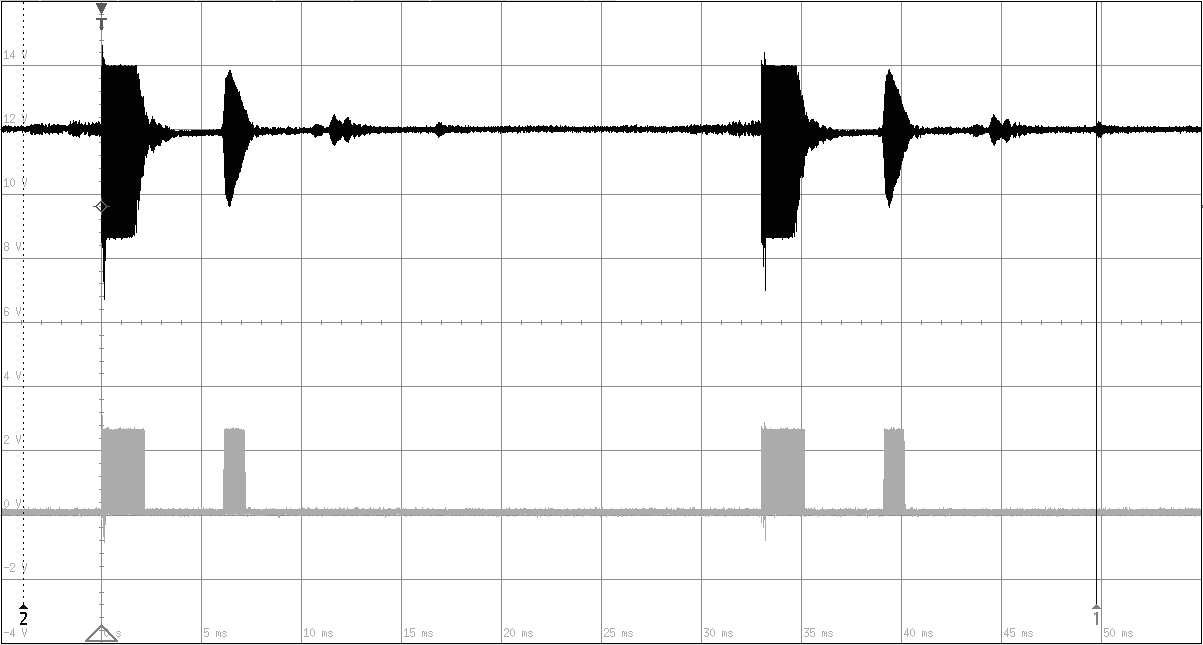
\includegraphics[width=1\textwidth%, draft
]{Abbildungen/MessungenP2/5V/1m.PNG}
\captionof{figure}{Signalverlauf bei 5V auf 1m Abstand}
\end{minipage}
\begin{minipage}{0.5\textwidth}
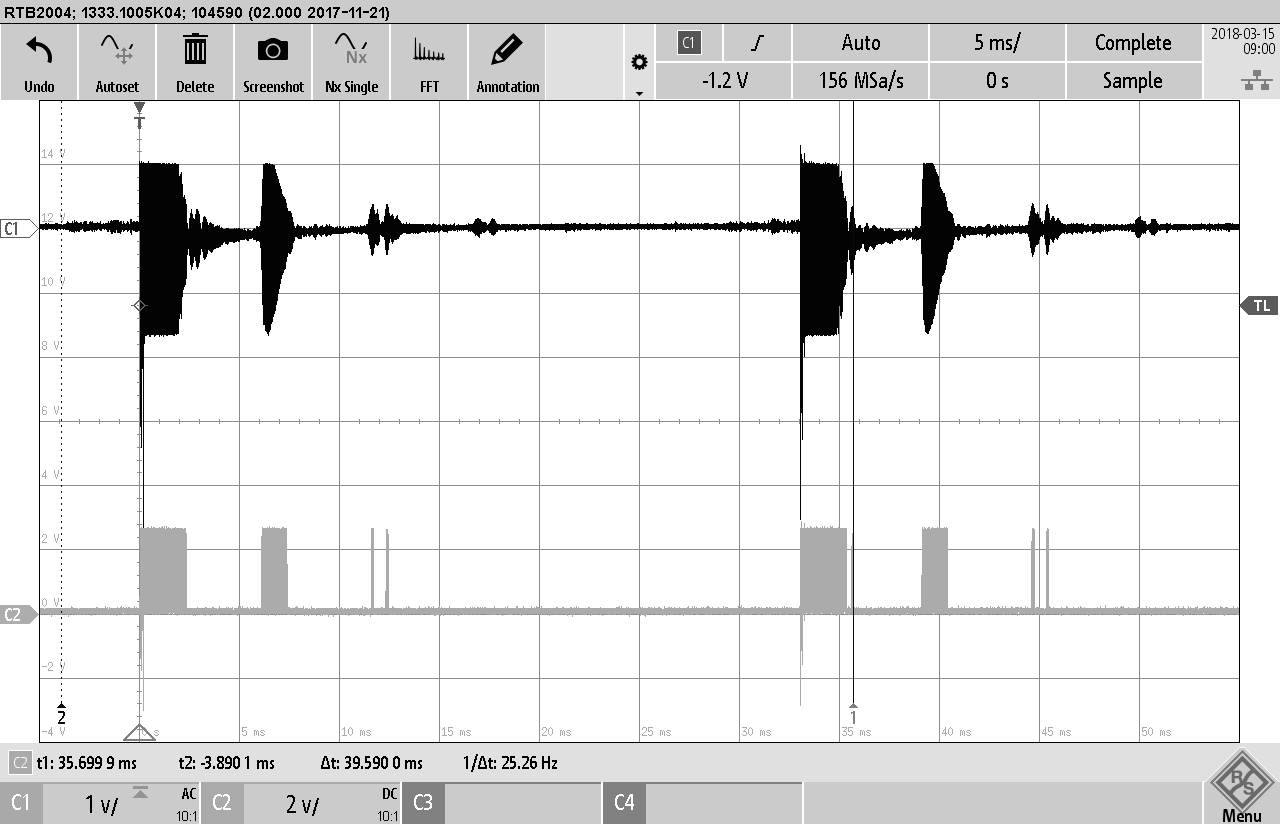
\includegraphics[width=1\textwidth%, draft
]{Abbildungen/MessungenP2/10V/1m.PNG}
\captionof{figure}{Signalverlauf bei 10V auf 1m Abstand}
\end{minipage}
\begin{minipage}{0.5\textwidth}
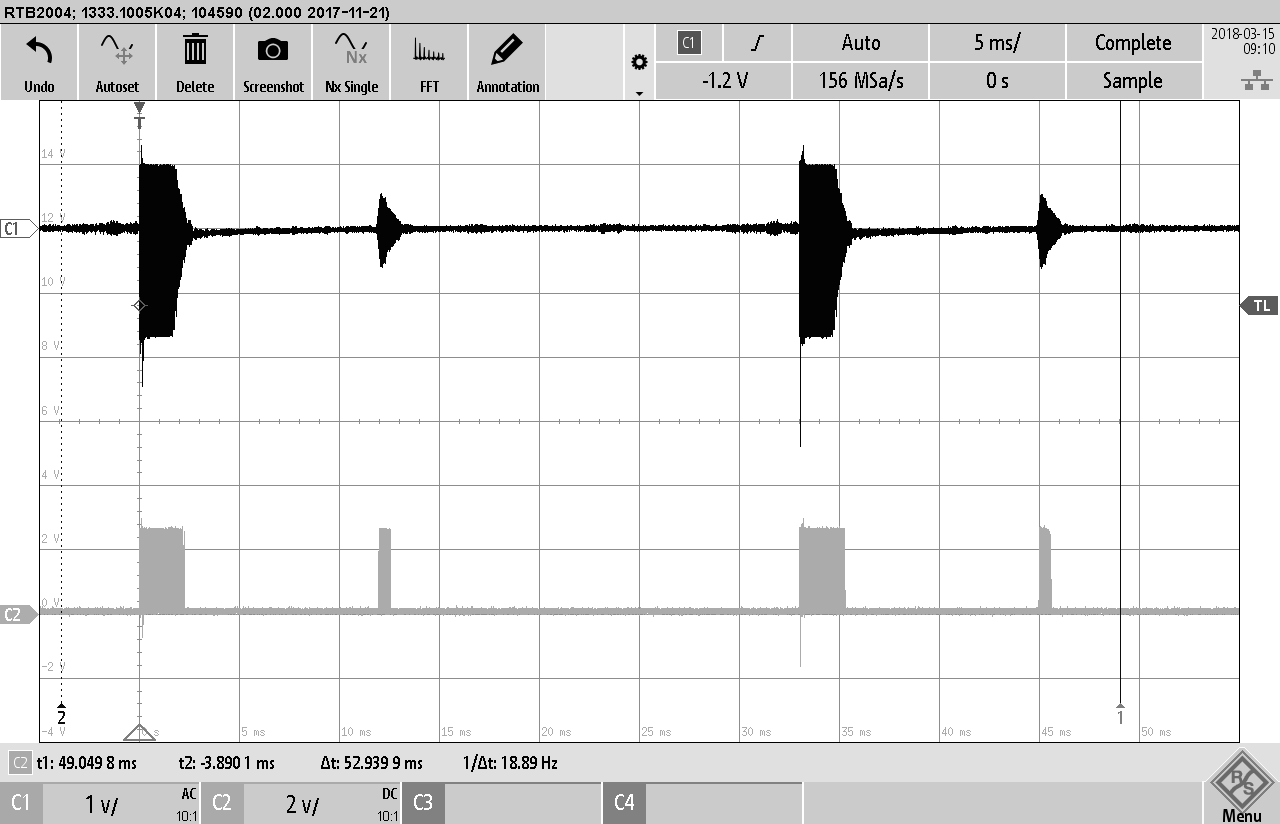
\includegraphics[width=1\textwidth%, draft
]{Abbildungen/MessungenP2/5V/2m.PNG}
\captionof{figure}{Signalverlauf bei 5V auf 2m Abstand}
\end{minipage}
\begin{minipage}{0.5\textwidth}
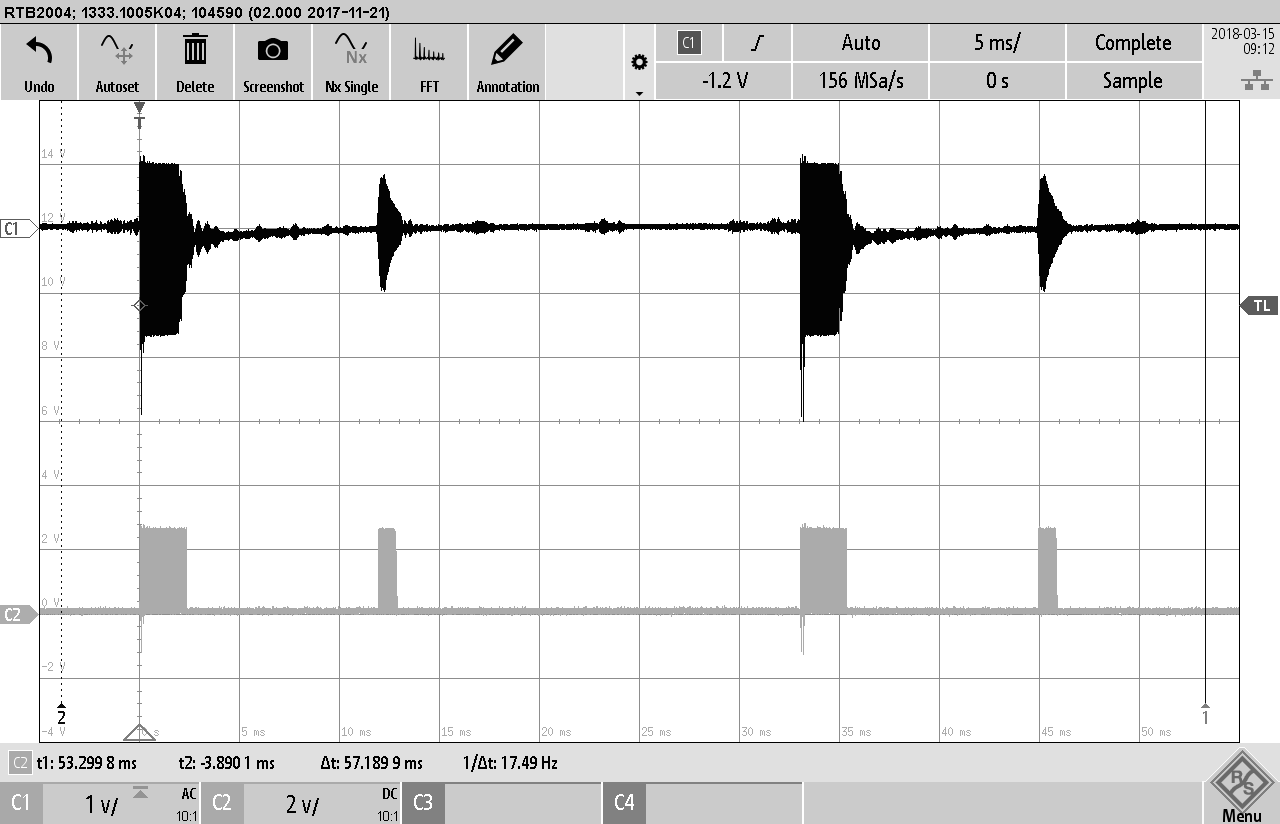
\includegraphics[width=1\textwidth%, draft
]{Abbildungen/MessungenP2/10V/2m.PNG}
\captionof{figure}{Signalverlauf bei 10V auf 2m Abstand}
\end{minipage}
\begin{minipage}{0.5\textwidth}
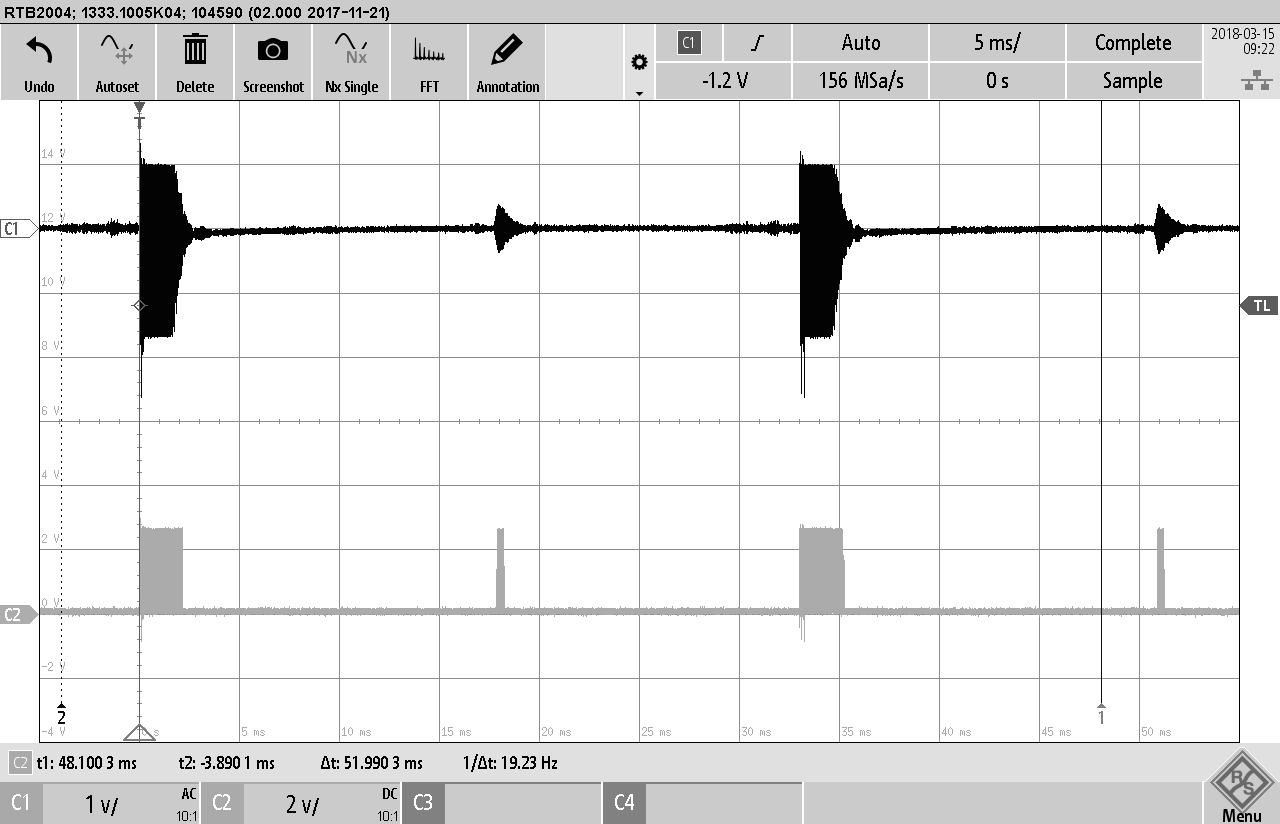
\includegraphics[width=1\textwidth%, draft
]{Abbildungen/MessungenP2/5V/3m.PNG}
\captionof{figure}{Signalverlauf bei 5V auf 3m Abstand}
\end{minipage}
\begin{minipage}{0.5\textwidth}
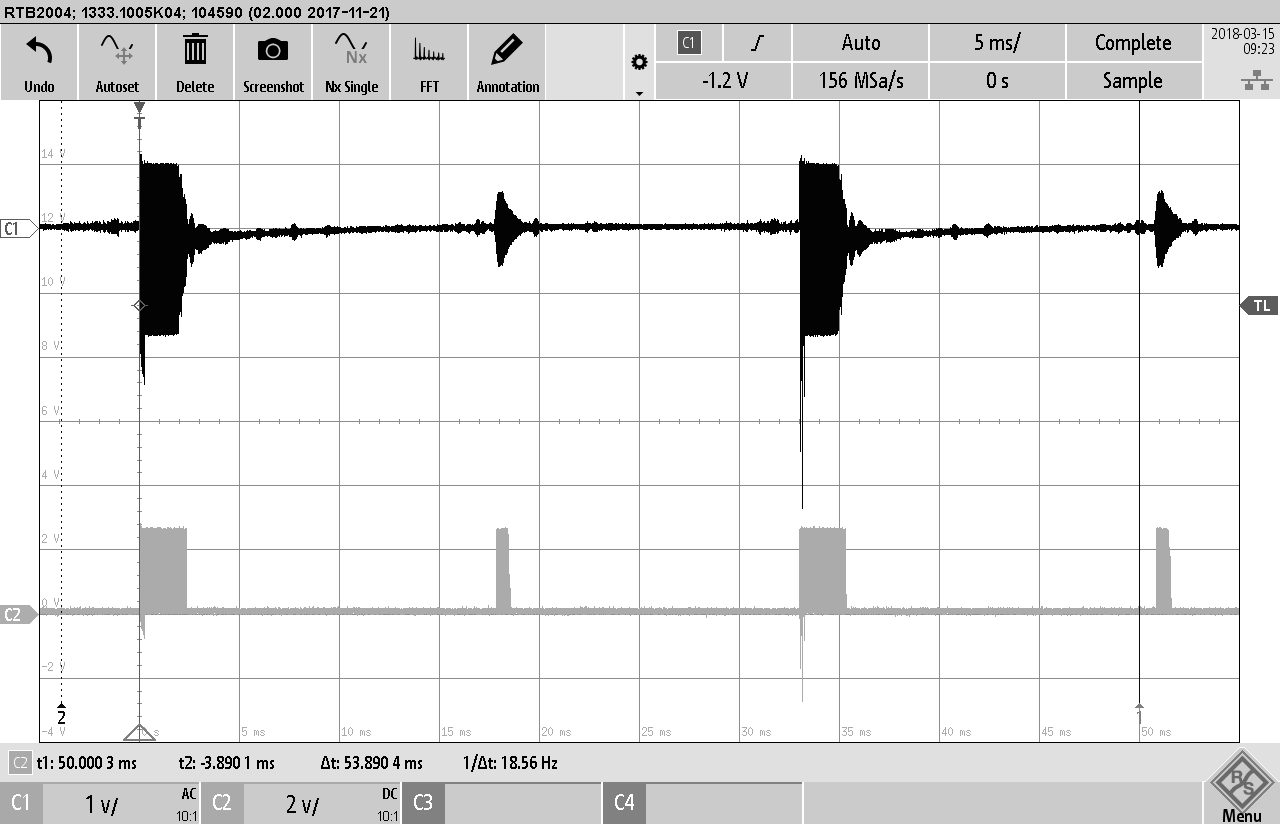
\includegraphics[width=1\textwidth%, draft
]{Abbildungen/MessungenP2/10V/3m.PNG}
\captionof{figure}{Signalverlauf bei 10V auf 3m Abstand}
\end{minipage}
\begin{minipage}{0.5\textwidth}
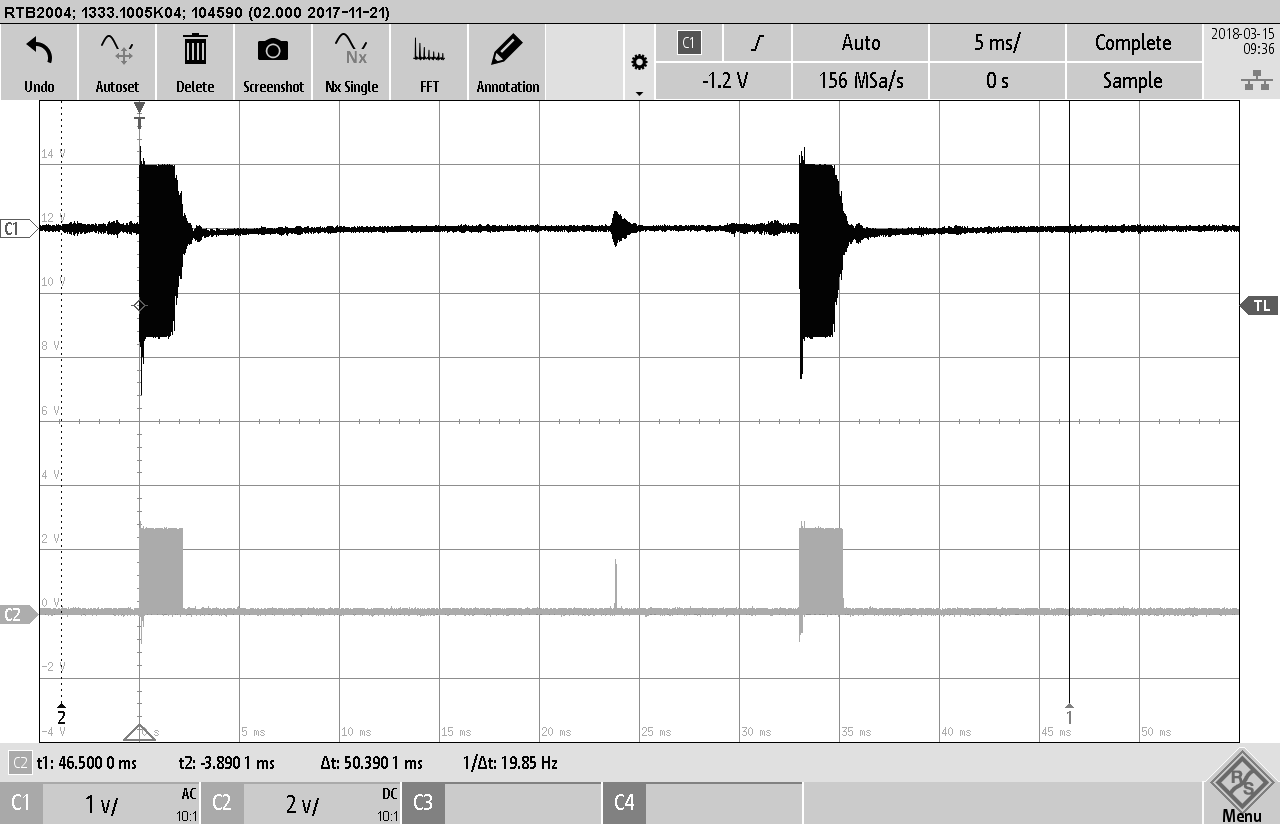
\includegraphics[width=1\textwidth%, draft
]{Abbildungen/MessungenP2/5V/4m.PNG}
\captionof{figure}{Signalverlauf bei 5V auf 4m Abstand}
\end{minipage}
\begin{minipage}{0.5\textwidth}
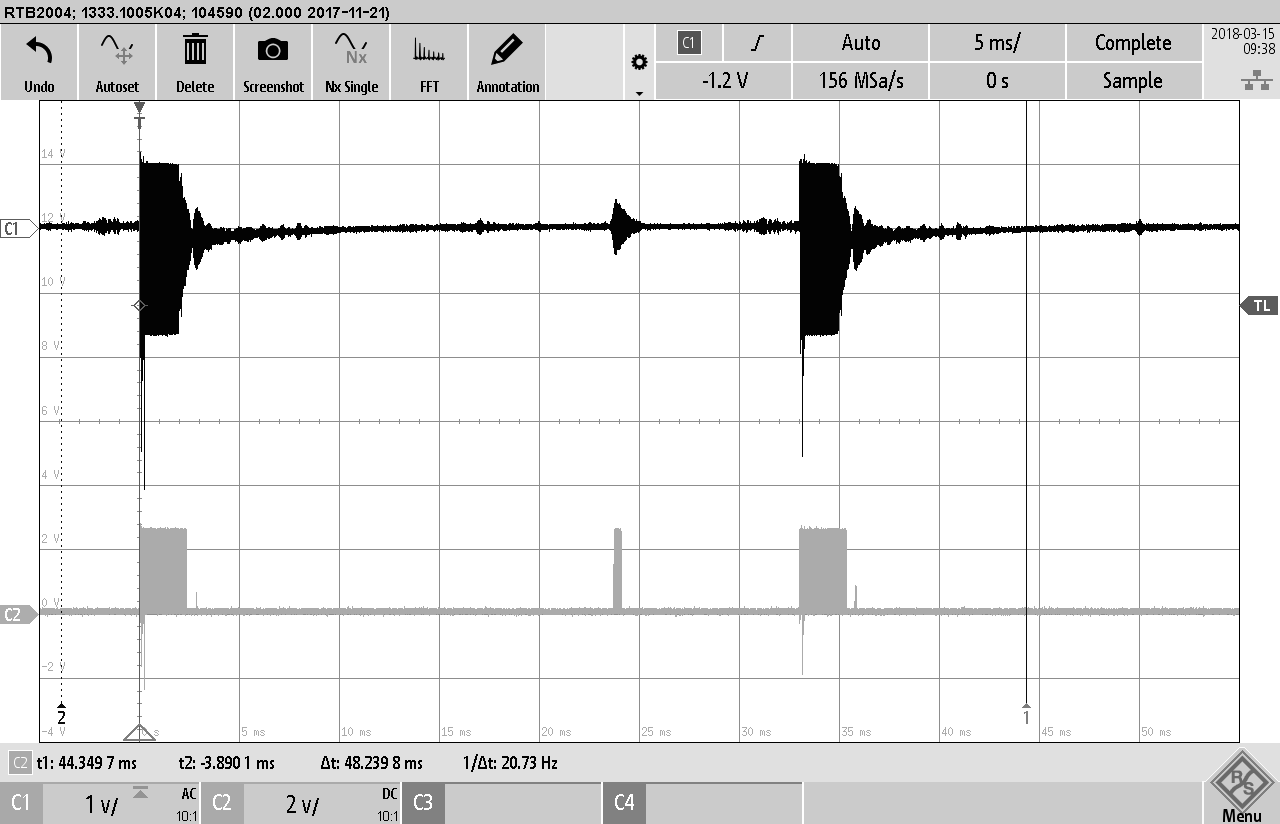
\includegraphics[width=1\textwidth%, draft
]{Abbildungen/MessungenP2/10V/4m.PNG}
\captionof{figure}{Signalverlauf bei 10V auf 4m Abstand}
\end{minipage}
\begin{minipage}{0.5\textwidth}
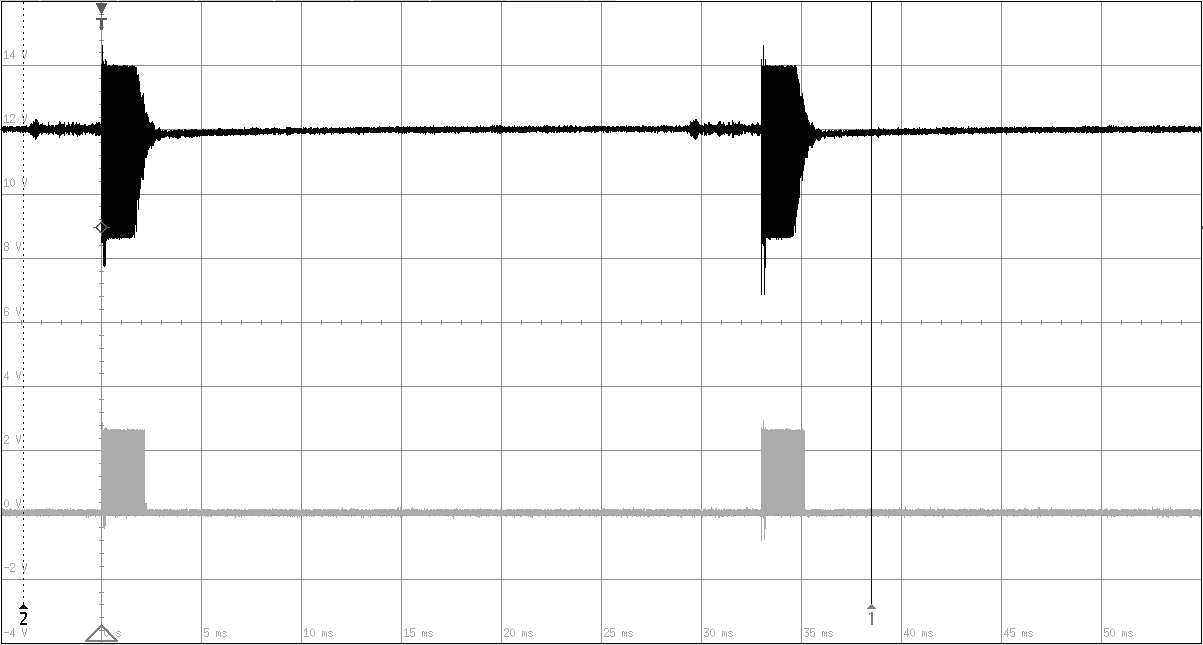
\includegraphics[width=1\textwidth%, draft
]{Abbildungen/MessungenP2/5V/5m.PNG}
\captionof{figure}{Signalverlauf bei 5V auf 5m Abstand}
\end{minipage}
\begin{minipage}{0.5\textwidth}
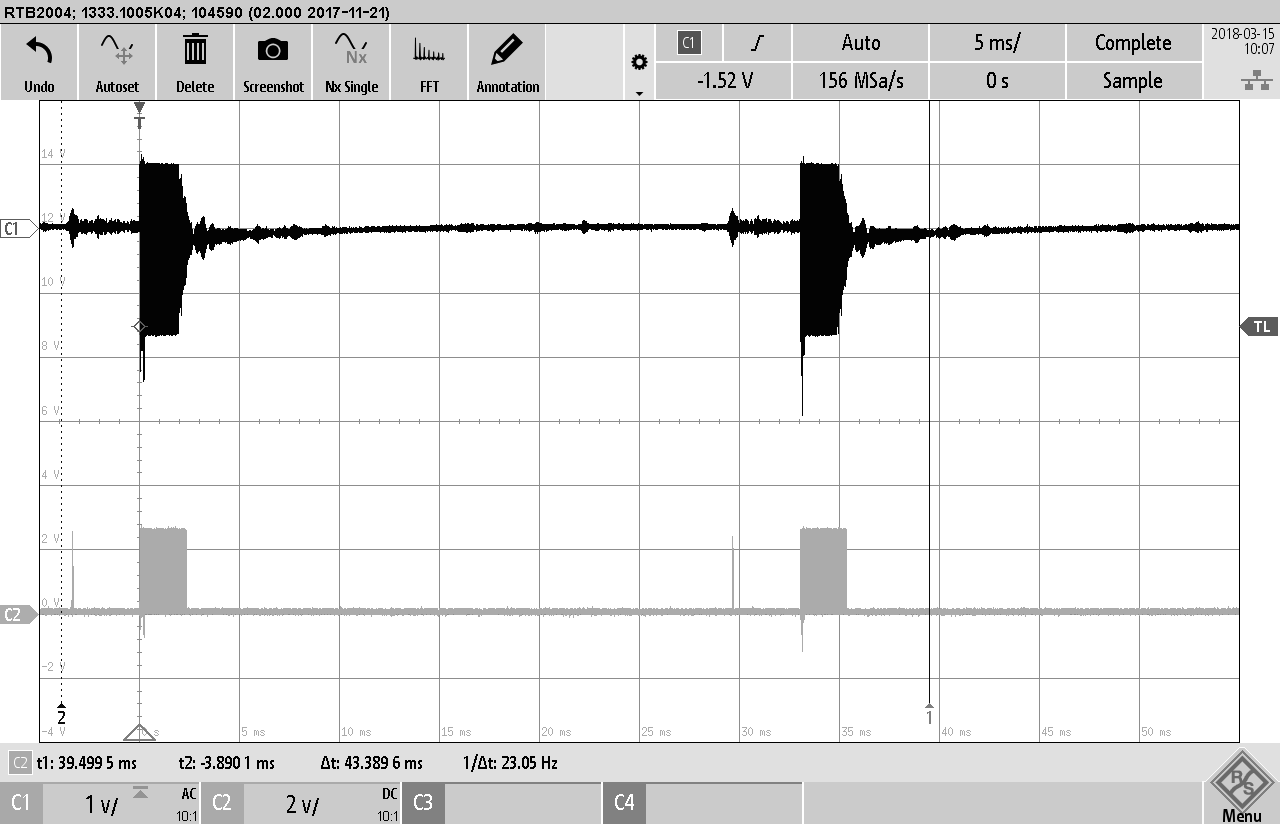
\includegraphics[width=1\textwidth%, draft
]{Abbildungen/MessungenP2/10V/5m.PNG}
\captionof{figure}{Signalverlauf bei 10V auf 5m Abstand}
\end{minipage}

\begin{minipage}{1\textwidth}
\begin{tabularx}{\textwidth}{|p{0.1\textwidth}|p{0.2\textwidth}|p{0.2\textwidth}|p{0.2\textwidth}|X|}
\hline
Entfernung [m]& Zeit bis Anfang Echo [ms] & Zeit bis Ende Echo [ms] & Errechnete Entfernung Anfang [m] & Errechnete Entfernung Ende [m]\\
\hline
1 & 6,11 & 7,23 & 1,0485 & 1,2407\\
\hline
1,5 & 9,02 & 9,89 & 1,5478 & 1,6971\\
\hline
2 & 11,97 & 12,76 & 2,0541 & 2,1896\\
\hline
2,5 & 14,88 & 15,5 & 2,5534 & 2,659\\
\hline
3 & 17,84 & 18,2 & 3,06134 & 3,1231\\
\hline
3,5 & 20,8 & 21,11 & 3,569 & 3,6225\\
\hline
4 & 23,71 & 23,81 & 4,0686 & 4,0858\\
\hline
4,5 & 26,61 & 26,73 & 4,5663 & 4,5869\\
\hline
5 & 29,59 & 29,68 & 5,0776 & 5,0961\\
\hline
\end{tabularx}
\captionof{table}{Entfernungsmessung bei 5V Sendespannung}
\label{tab:Entfernungsmessung5V}
\begin{tabularx}{\textwidth}{|p{0.1\textwidth}|p{0.2\textwidth}|p{0.2\textwidth}|p{0.2\textwidth}|X|}
\hline
Entfernung [m]& Zeit bis Anfang Echo [ms] & Zeit bis Ende Echo [ms] & Errechnete Entfernung Anfang [m] & Errechnete Entfernung Ende [m]\\
\hline
1 & 6,07 & 7,37 & 1,0416 & 1,2647\\
\hline
1,5 & 8,99 & 10,02 & 1,5427 & 1,7194\\
\hline
2 & 11,94 & 12,9 & 2,0489 & 2,2136\\
\hline
2,5 & 14,83 & 15,7 & 2,5448 & 2,6941\\
\hline
3 & 17,8 & 18,48 & 3,0545 & 3,1712\\
\hline
3,5 & 20,7 & 21,36 & 3,5521 & 3,6654\\
\hline
4 & 23,62 & 24 & 4,0532 & 4,1184\\
\hline
4,5 & 26,55 & 26,9 & 4,5560 & 4,6160\\
\hline
5 & 29,5 & 29,9 & 5,0622 & 5,1308\\
\hline
\end{tabularx}
\captionof{table}{Entfernungsmessung bei 10V Sendespannung}
\label{tab:Entfernungsmessung10V}
\end{minipage}\\
\chapter{Quellenangaben}
https://www.eurocircuits.com/pcb-design-guidelines/ //PCB RUles
http://rn-wissen.de/wiki/index.php/Abblockkondensator  //Abblockkondensator
https://www.elektronikpraxis.vogel.de/sieben-suenden-beim-leiterplatten-design-a-356703/
https://www.mikrocontroller.net/articles/Richtiges_Designen_von_Platinenlayouts
https://www.mikrocontroller.net/articles/Schaltplan_richtig_zeichnen//(Part Schaltplan 1.3.1) 15.03.2018
https://www.infineon.com/cms/en/product/microcontroller/32-bit- industrial-microcontroller- based-
on-arm- cortex-m/32- bit-xmc1000- industrial-microcontroller- arm-cortex- m0/\#\\

\listoftables


\end{document}


